\input{../utils/preamble}
\createdgmtitle{11}
%--------------------------------------------------------------------------------
\begin{document}
%--------------------------------------------------------------------------------
\begin{frame}
%\thispagestyle{empty}
\titlepage
\end{frame}
%=======
\begin{frame}{Spectral Normalization GAN}
	How else could we enforce Lipschitzness?
	\begin{block}{Fact 1}
		Let denote by $\sigma(\bA)$ a spectral norm of matrix $\bA$.
		\[
			\sigma(\bA) = \max_{\bh \neq 0} \frac{\|\bA \bh\|_2}{\|\bh\|_2} = \max_{\|\bh\|_2 \leq 1} \| \bA \bh \|_2 = \lambda_{\text{max}}(\bA),
		\]
		where $\lambda_{\text{max}}(\bA)$ is the largest singular value of $\bA$. \\
		By definition, Lipschitz norm is 
		\[
			\| \mathbf{g} \|_L = \sup_\bx \sigma( \nabla \mathbf{g}(\bx))
		\]
	\end{block}
	\vspace{-0.5cm}
	\begin{block}{Fact 2}
		Lipschitz norm of superposition is bounded above by product of Lipschitz norms
		\vspace{-0.2cm}
		\[
			\| \mathbf{g}_1 \circ \mathbf{g}_2 \|_L \leq \| \mathbf{g}_1 \|_L \cdot \| \mathbf{g}_2\|_L
		\]
	\end{block}
	\myfootnotewithlink{https://arxiv.org/abs/1802.05957}{Miyato T. et al. Spectral Normalization for Generative Adversarial Networks, 2018}
\end{frame}
%=======
\begin{frame}{Spectral Normalization GAN}
	Let consider the critic $f(\bx, \bphi)$ of the following form:
	\[
		f(\bx, \bphi) = \bW_{K+1} a_K (\bW_K a_{K-1}(\dots a_1(\bW_1 \bx) \dots)).
	\]
	This feedforward network is a superposition of simple functions.
	\begin{itemize}
		\item $a_k$ is a pointwise nonlinearities. We assume that $\| a_k \|_L = 1$ (it holds for ReLU).
		\item $\mathbf{g}(\bh) = \bW \bh$ is a linear transformation ($\nabla \mathbf{g}(\bx) = \bW$).
		\[
			\| \mathbf{g} \|_L = \sup_\bx \sigma( \nabla \mathbf{g}(\bx)) = \sigma(\bW).
		\]
	\end{itemize}
	\vspace{-0.3cm}
	\begin{block}{Critic spectral norm}
		\vspace{-0.3cm}
		\[
			\| f \|_L \leq \| \bW_{K+1}\| \cdot \prod_{k=1}^K  \| a_k \|_L \cdot \| \bW_k \| = \prod_{k=1}^{K+1} \sigma(\bW_k).
		\]
		\vspace{-0.2cm}
	\end{block}
	If we replace the weights in the critic $f(\bx, \bphi)$ by $\bW^{SN}_k = \bW_k / \sigma(\bW_k)$, we will get $\| f\|_L \leq 1.$ \\
	
	\myfootnotewithlink{https://arxiv.org/abs/1802.05957}{Miyato T. et al. Spectral Normalization for Generative Adversarial Networks, 2018}
\end{frame}
%=======
\begin{frame}{Spectral Normalization GAN}
	How to compute $\sigma(\bW)$? \\
	 If we apply singular value decomposition to compute the $\sigma(\bW)$ at each round of the algorithm, the algorithm becomes intractable.
	 
	 \begin{block}{Power iteration}
	 	\begin{itemize}
	 		\item $\bu_0$ -- random vector.
	 		\item for $k = 0, \dots, n - 1$: ($n$ is a large enough number of steps)
	 		\[
	 			\bv_{k+1} = \frac{\bW^T \bu_{k}}{\| \bW^T \bu_{k} \|}, \quad \bu_{k+1} = \frac{\bW \bv_{k+1}}{\| \bW \bv_{k+1} \|}
	 		\]
	 		\item approximate the spectral norm
	 		\[
	 			\sigma(\bW) \approx \bu_{n}^T \bW \bv_{n}
	 		\]
	 	\end{itemize}
	 \end{block}

	\myfootnotewithlink{https://arxiv.org/abs/1802.05957}{Miyato T. et al. Spectral Normalization for Generative Adversarial Networks, 2018}
\end{frame}
%=======
\begin{frame}{Spectral Normalization GAN}
	\begin{figure}
		\centering
		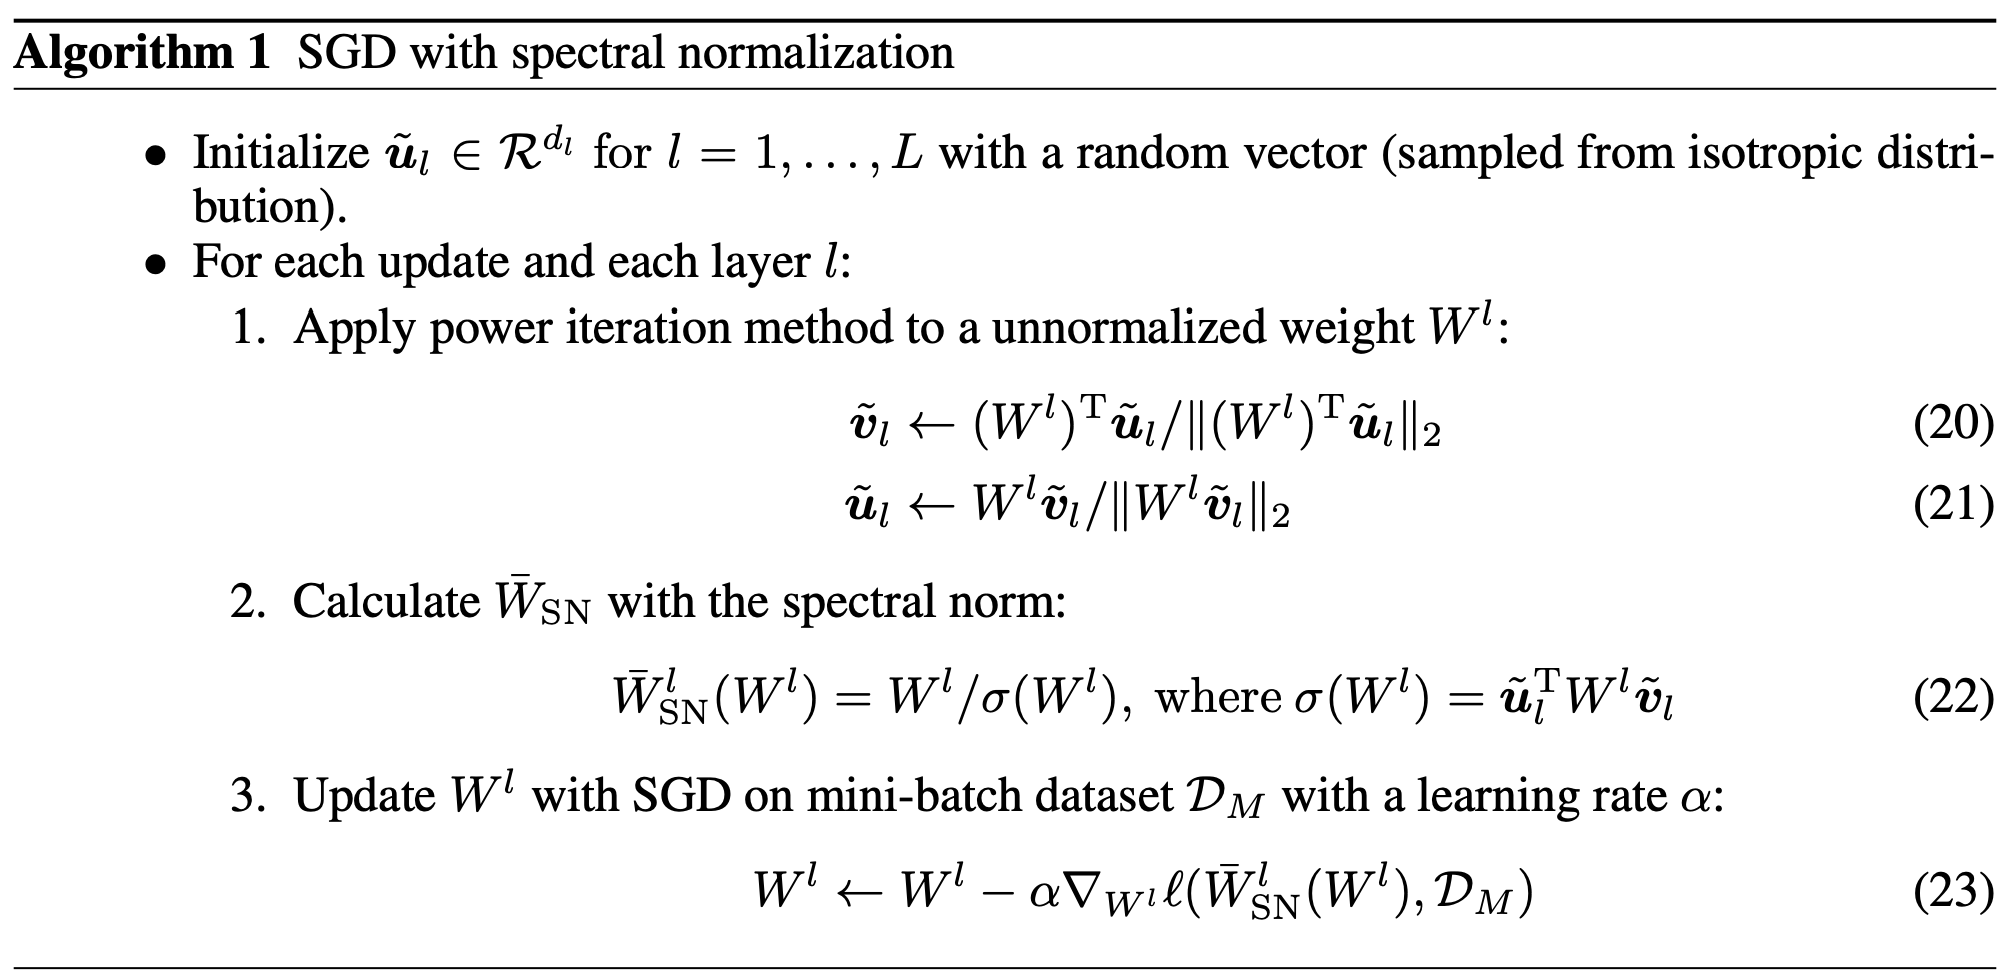
\includegraphics[width=0.85\linewidth]{figs/sngan_pseudocode}
	\end{figure}
	\begin{figure}
		\centering
		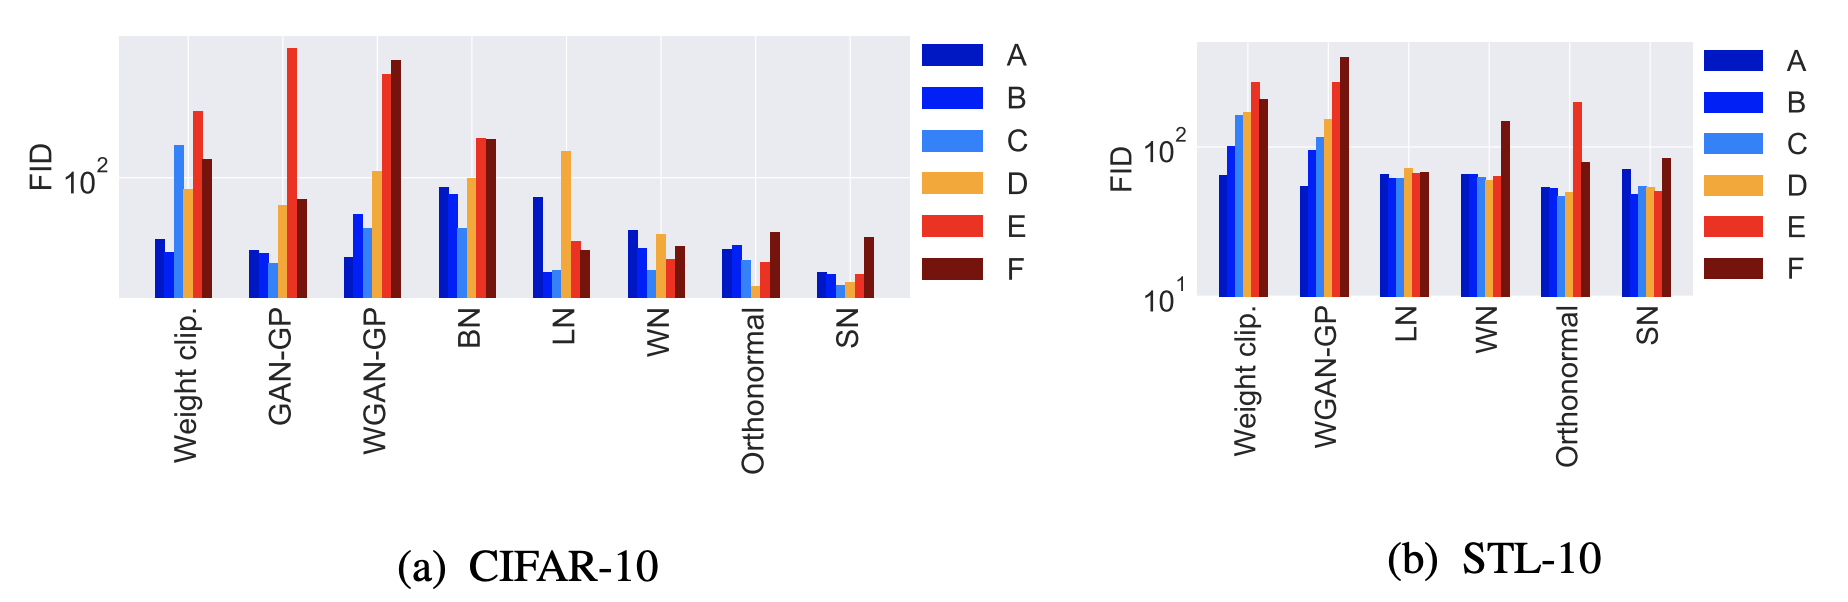
\includegraphics[width=0.85\linewidth]{figs/sngan_fids}
	\end{figure}

	\myfootnotewithlink{https://arxiv.org/abs/1802.05957}{Miyato T. et al. Spectral Normalization for Generative Adversarial Networks, 2018}
\end{frame}
%=======
\begin{frame}{Divergences}
	\begin{block}{What do we have?}
		\begin{itemize}
			\item Forward KL divergence in maximum likelihood estimation
			\item Reverse KL in variational inference
			\item JS divergence in  vanilla gan
			\item Wasserstein distance in WGAN
		\end{itemize}
	\end{block}
	\begin{block}{What is a divergence?}
		Let $\cS$ be the set of all possible probability distributions. Then $D: \cS \times \cS \rightarrow \bbR$ is a divergence if 
		\begin{itemize}
			\item $D(\pi || p) \geq 0$ for all $\pi, p \in \cS$;
			\item $D(\pi || p) = 0$ if and only if $\pi \equiv p$.
		\end{itemize}
	\end{block}
	\begin{block}{General divergence minimization task}
		\vspace{-0.3cm}
		\[
			\min_p D(\pi || p)
		\]
		\vspace{-0.5cm}
	\end{block}
\end{frame}
%=======
\begin{frame}{f-divergence family}
	
	\begin{block}{f-divergence}
		\vspace{-0.3cm}
		\[
		D_f(\pi || p) = \bbE_{p(\bx)}  f\left( \frac{\pi(\bx)}{p(\bx)} \right)  = \int p(\bx) f\left( \frac{\pi(\bx)}{p(\bx)} \right) d \bx.
		\]
		Here $f: \bbR_+ \rightarrow \bbR$ is a convex, lower semicontinuous function satisfying $f(1) = 0$.
	\end{block}
	\begin{figure}
		\centering
		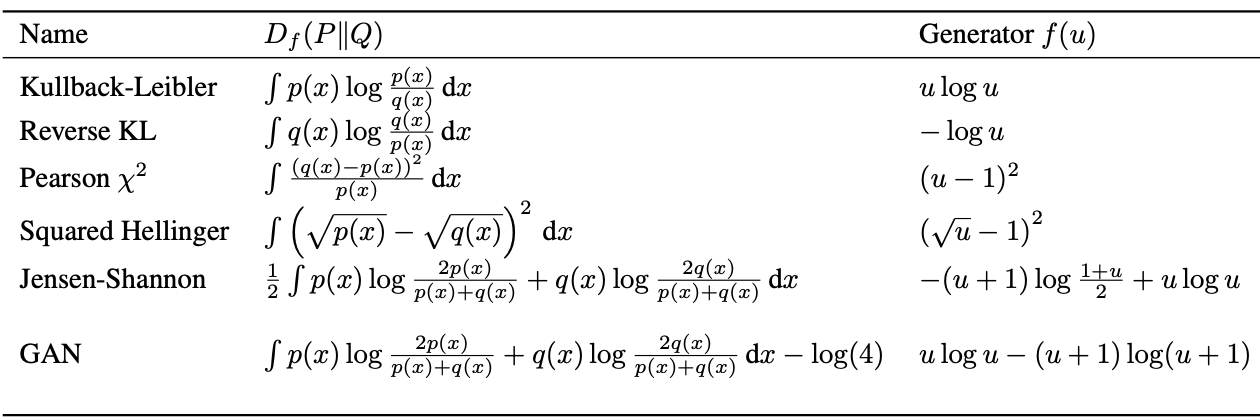
\includegraphics[width=\linewidth]{figs/f_divs}
	\end{figure}
	\myfootnotewithlink{https://arxiv.org/abs/1606.00709}{Nowozin S., Cseke B., Tomioka R. f-GAN: Training Generative Neural Samplers using Variational Divergence Minimization, 2016}
\end{frame}
%=======
\begin{frame}{f-divergence family}
	\vspace{-0.2cm}
	\begin{block}{Fenchel conjugate}
		\vspace{-0.7cm}
		\[
		f^*(t) = \sup_{u \in \text{dom}_f} \left( ut - f(u) \right), \quad f(u) = \sup_{t \in \text{dom}_{f^*}} \left( ut - f^*(t) \right)
		\]
		\vspace{-0.5cm}
	\end{block}
	\textbf{Important property:} $ f^{**} = f$ for convex $f$.
	\begin{block}{f-divergence}
		\vspace{-0.8cm}
		\begin{multline*}
			D_f(\pi || p) = \bbE_{p(\bx)}  f\left( \frac{\pi(\bx)}{p(\bx)} \right)  = \int p(\bx) f\left( \frac{\pi(\bx)}{p(\bx)} \right) d \bx = \\ = \int p(\bx) \sup_{t \in \text{dom}_{f^*}} \left( \frac{\pi(\bx)}{p(\bx)} t - f^*(t) \right) d \bx = \\ 
			= \int \sup_{t \in \text{dom}_{f^*}} \left( \pi(\bx)t - p(\bx) f^*(t) \right) d \bx .
		\end{multline*}
		\vspace{-0.6cm}
	\end{block}
	Here we seek value of $t$, which gives us maximum value of $ \pi(\bx)t - p(\bx) f^*(t)$, for each data point $\bx$.
	\myfootnotewithlink{https://arxiv.org/abs/1606.00709}{Nowozin S., Cseke B., Tomioka R. f-GAN: Training Generative Neural Samplers using Variational Divergence Minimization, 2016}
\end{frame}
%=======
\begin{frame}{f-divergence family}
	\vspace{-0.4cm}
	\begin{block}{f-divergence}
		\vspace{-0.3cm}
		\[
		D_f(\pi || p) = \bbE_{p(\bx)}  f\left( \frac{\pi(\bx)}{p(\bx)} \right)  = \int p(\bx) f\left( \frac{\pi(\bx)}{p(\bx)} \right) d \bx.
		\]
		\vspace{-0.4cm}
	\end{block}
	\begin{block}{Variational f-divergence estimation}
		\vspace{-0.8cm}
		\begin{multline*}
			D_f(\pi || p)  = \int \sup_{t \in \text{dom}_{f^*}} \left( \pi(\bx)t - p(\bx) f^*(t) \right) d \bx \geq \\
			 \geq \sup_{T \in \cT} \int \left( \pi(\bx)T(\bx) - p(\bx) f^*(T(\bx)) \right) d \bx = \\
			 = \sup_{T \in \cT} \left[\bbE_{\pi}T(\bx) -  \bbE_p f^*(T(\bx)) \right]
		\end{multline*}
	\vspace{-0.6cm}
	\end{block}
	This is a lower bound because of Jensen-Shannon inequality and restricted class of functions $\cT: \cX \rightarrow \bbR$.
	
	\textbf{Note:} To evaluate lower bound we only need samples from $\pi(\bx)$ and $p(\bx)$. Hence, we could fit implicit generative model.
	\myfootnotewithlink{https://arxiv.org/abs/1606.00709}{Nowozin S., Cseke B., Tomioka R. f-GAN: Training Generative Neural Samplers using Variational Divergence Minimization, 2016}
\end{frame}
%=======
\begin{frame}{f-divergence family}
	\begin{block}{Variational divergence estimation}
		\[
			D_f(\pi || p) \geq \sup_{T \in \cT} \left[\bbE_{\pi}T(\bx) -  \bbE_p f^*(T(\bx)) \right]
		\]
		The lower bound is tight for $T^*(\bx) = f'\left( \frac{\pi(\bx)}{p(\bx)} \right)$.
	\end{block}
	\begin{figure}
		\centering
		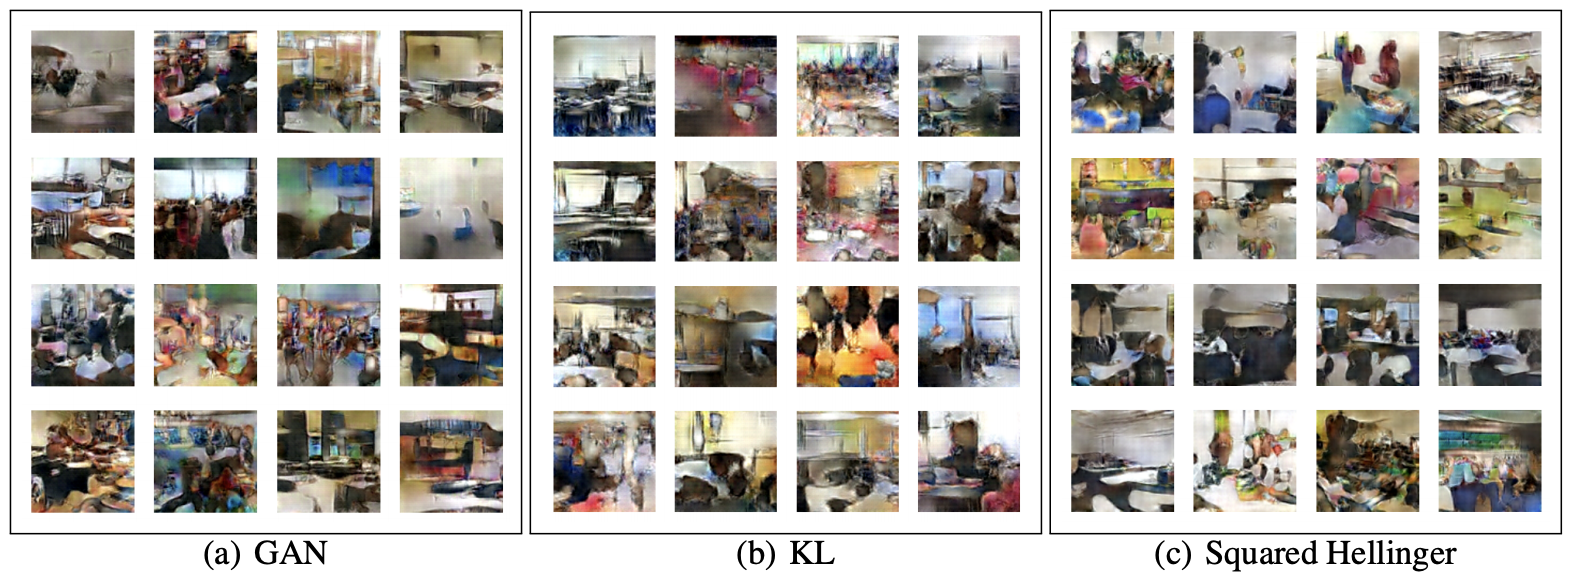
\includegraphics[width=1.0\linewidth]{figs/f_div_results}
	\end{figure}

	\myfootnotewithlink{https://arxiv.org/abs/1606.00709}{Nowozin S., Cseke B., Tomioka R. f-GAN: Training Generative Neural Samplers using Variational Divergence Minimization, 2016}
\end{frame}
%=======
\begin{frame}{Evaluation of likelihood-free models}
	How to evaluate generative models?
	\begin{block}{Likelihood-based models}
		\begin{itemize}
			\item Split data to train/val/test.
			\item Fit model on the train part.
			\item Tune hyperparameters on the validation part.
			\item Evaluate generalization by reporting likelihoods on the test set.
		\end{itemize}
	\end{block}
	\begin{block}{Not all models have tractable likelihoods}
		\begin{itemize}
			\item VAE: compare ELBO values.
			\item GAN: ???
		\end{itemize}
	\end{block}
\end{frame}
%=======
\begin{frame}{Evaluation of likelihood-free models}
	Let take some pretrained image classification model to get the conditional label distribution $p(y | \bx)$ (e.g. ImageNet classifier).
	\begin{block}{What do we want from samples?}
		\begin{itemize}
			\item \textbf{Sharpness}
			\begin{figure}
				\centering
				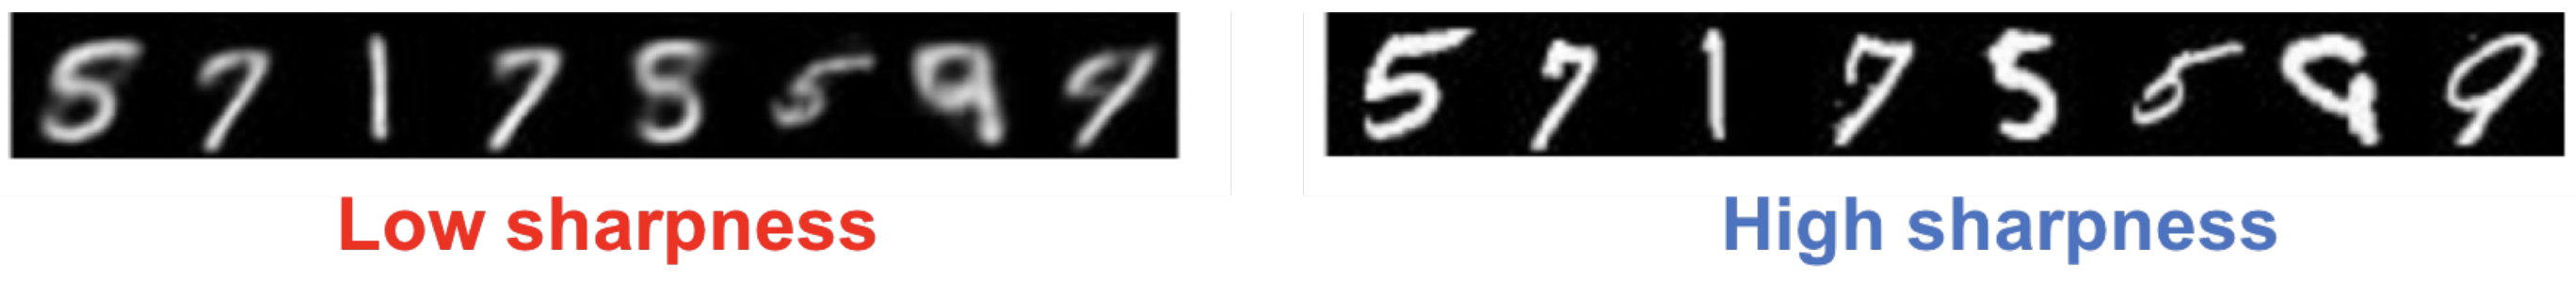
\includegraphics[width=0.9\linewidth]{figs/sharpness}
			\end{figure}
			The conditional distribution $p(y | \bx)$ should have low entropy (each image $\bx$ should have distinctly recognizable object).
			\item \textbf{Diversity}
			\begin{figure}
				\centering
				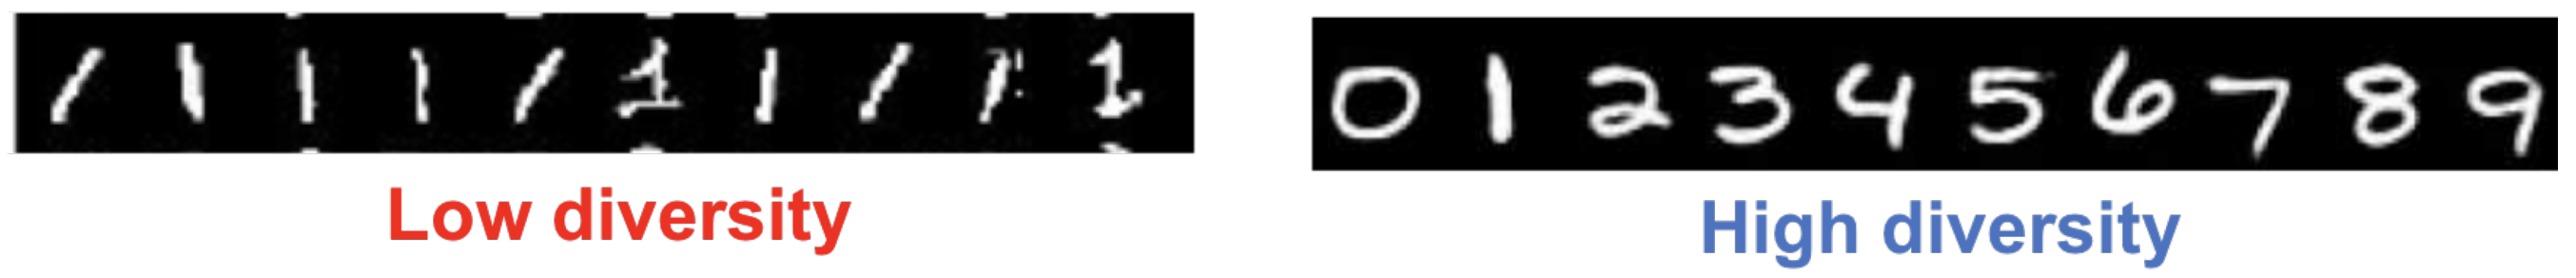
\includegraphics[width=0.9\linewidth]{figs/diversity}
			\end{figure}
			The marginal distribution $p(y) = \int p(y | \bx) p(\bx) d \bx$ should have high entropy (there should be as many classes generated as possible).
		\end{itemize}
	\end{block}
	\myfootnotewithlink{https://deepgenerativemodels.github.io}{image credit: https://deepgenerativemodels.github.io}
\end{frame}
%=======
\begin{frame}{Evaluation of likelihood-free models}
	\begin{block}{What do we want from samples?}
		\begin{itemize}
			\item \textbf{Sharpness.}
			The conditional distribution $p(y | \bx)$ should have low entropy (each image $\bx$ should have distinctly recognizable object).
			\item \textbf{Diversity.}
			The marginal distribution $p(y) = \int p(y | \bx) p(\bx) d \bx$ should have high entropy (there should be as many classes generated as possible).
		\end{itemize}
	\end{block}
	\begin{figure}
		\centering
		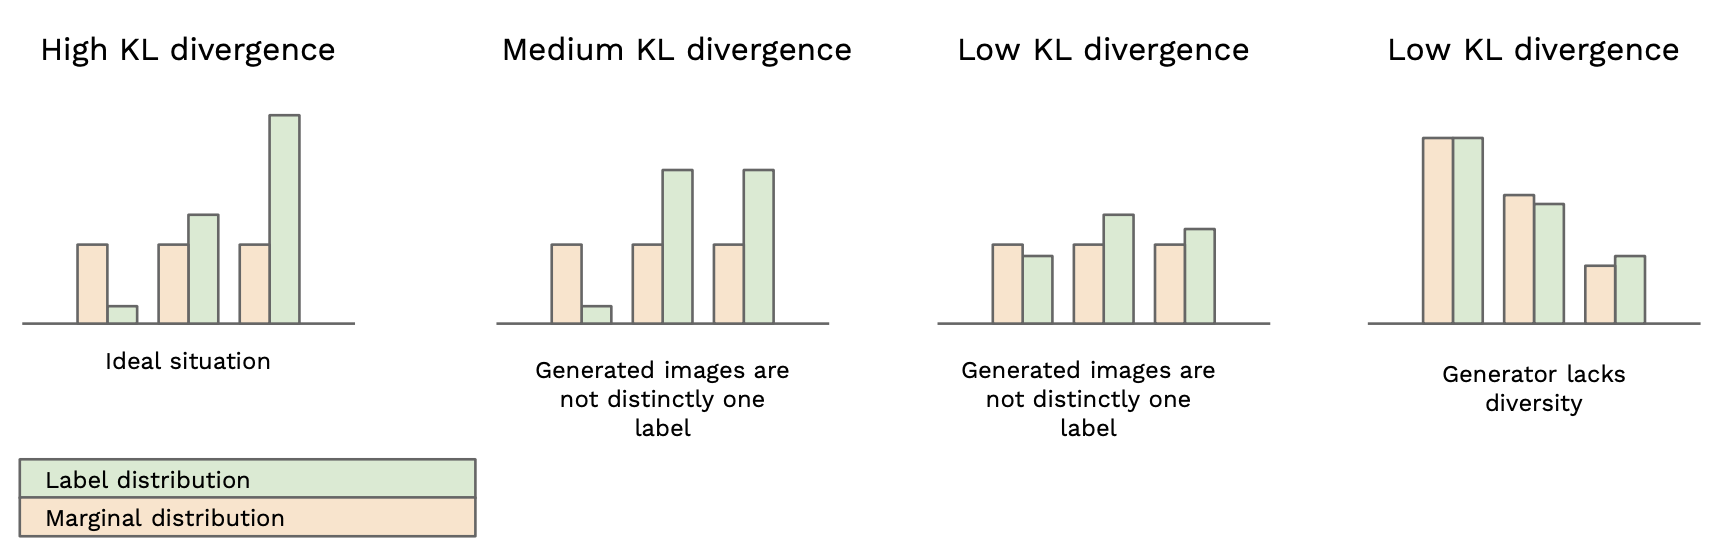
\includegraphics[width=1.0\linewidth]{figs/is_toy}
	\end{figure}
	\myfootnotewithlink{https://medium.com/octavian-ai/a-simple-explanation-of-the-inception-score-372dff6a8c7a}{image credit: https://medium.com/octavian-ai/a-simple-explanation-of-the-inception-score-372dff6a8c7a}
\end{frame}
%=======
\begin{frame}{Evaluation of likelihood-free models}
		\begin{block}{What do we want from samples?}
		\begin{itemize}
			\item Sharpness $\Rightarrow$ low $H(y | \bx) = - \sum_{y} \int_{\bx} p(y, \bx) \log p(y | \bx) d\bx$.
			\item Diversity $\Rightarrow$ high $H(y)  = - \sum_{y} p(y) \log p(y)$.
		\end{itemize}
	\end{block}
	\begin{block}{Inception Score}
		\vspace{-0.3cm}
		\footnotesize
		\begin{align*}
			IS &= \exp(H(y) - H(y | \bx)) \\ 
			&= \exp \left( - \sum_{y} p(y) \log p(y) + \sum_{y} \int_{\bx} p(y, \bx) \log p(y | \bx) d\bx\right) \\
			&= \exp \left( \sum_{y} \int_{\bx} p(y, \bx) \log \frac{p(y | \bx)}{p(y)} d\bx\right) \\ 
			&= \exp \left( \bbE_{\bx} \sum_{y} p(y | \bx) \log \frac{p(y | \bx)}{p(y)} \right) = \exp \left( \bbE_{\bx} KL(p(y | \bx) || p(y)) \right)
		\end{align*}
	\end{block}
	\myfootnotewithlink{https://arxiv.org/abs/1606.03498}{Salimans T. et al. Improved Techniques for Training GANs, 2016}
\end{frame}
%=======
\begin{frame}{Evaluation of likelihood-free models}
	\begin{block}{Inception Score}
		\vspace{-0.1cm}
		\[
			IS =  \exp \left( \bbE_{\bx} KL(p(y | \bx) || p(y)) \right)
		\]
		\vspace{-0.1cm}
	\end{block}
	\begin{block}{IS limitations}
		\begin{itemize}
			\item Inception score depends on the quality of the pretrained classifier $p(y | \bx)$.
			\item If generator produces images with a different set of labels from the classifier training set, IS will be low.
			\item If the generator produces one image per class, the IS will be perfect (there is no measure of intra-class diversity).
			\item IS only require samples from the generator and do not take into account the desired data distribution $\pi(\bx)$ directly (only implicitly via a classifier).
		\end{itemize}
	\end{block}
	\myfootnotewithlink{https://arxiv.org/abs/1801.01973}{Barratt S., Sharma R. A Note on the Inception Score, 2018}
\end{frame}
%=======
\begin{frame}{Evaluation of likelihood-free models}
	\begin{block}{Theorem}
		If $\pi(\bx)$ and $p(\bx | \btheta)$ has moment generation functions then
		\[
			\pi(\bx) = p(\bx | \btheta) \, \Leftrightarrow \, \bbE_{\pi} \bx^k = \bbE_{p} \bx^k, \quad \forall k \geq 1.
		\]
	\end{block}
	This is intractable to calculate all moments.
	\begin{block}{Frechet Inception Distance}
		\vspace{-0.1cm}
		\[
			D^2 (\pi, p) = \| \mathbf{m}_{\pi} - \mathbf{m}_{p}\|_2^2 + \text{Tr} \left( \bC_{\pi} + \bC_p - 2 \sqrt{\bC_{\pi} \bC_p} \right)
		\]
	\end{block}
	\begin{itemize}
		\item $\mathbf{m}_{\pi}$, $\bC_{\pi} $ are mean vector and covariance matrix of feature representations for real samples from $\pi(\bx)$
		\item $\mathbf{m}_{p}$, $\bC_p$ are mean vector and covariance matrix of feature representations for generated samples from $p(\bx | \btheta)$.
		\item Representations are outputs of intermediate layer from pretrained classification model.
	\end{itemize} 

	\myfootnotewithlink{https://arxiv.org/abs/1706.08500}{Heusel M. et al. GANs Trained by a Two Time-Scale Update Rule Converge to a Local Nash Equilibrium, 2017}
\end{frame}
%=======
\begin{frame}{Evaluation of likelihood-free models}
	\begin{figure}
		\centering
		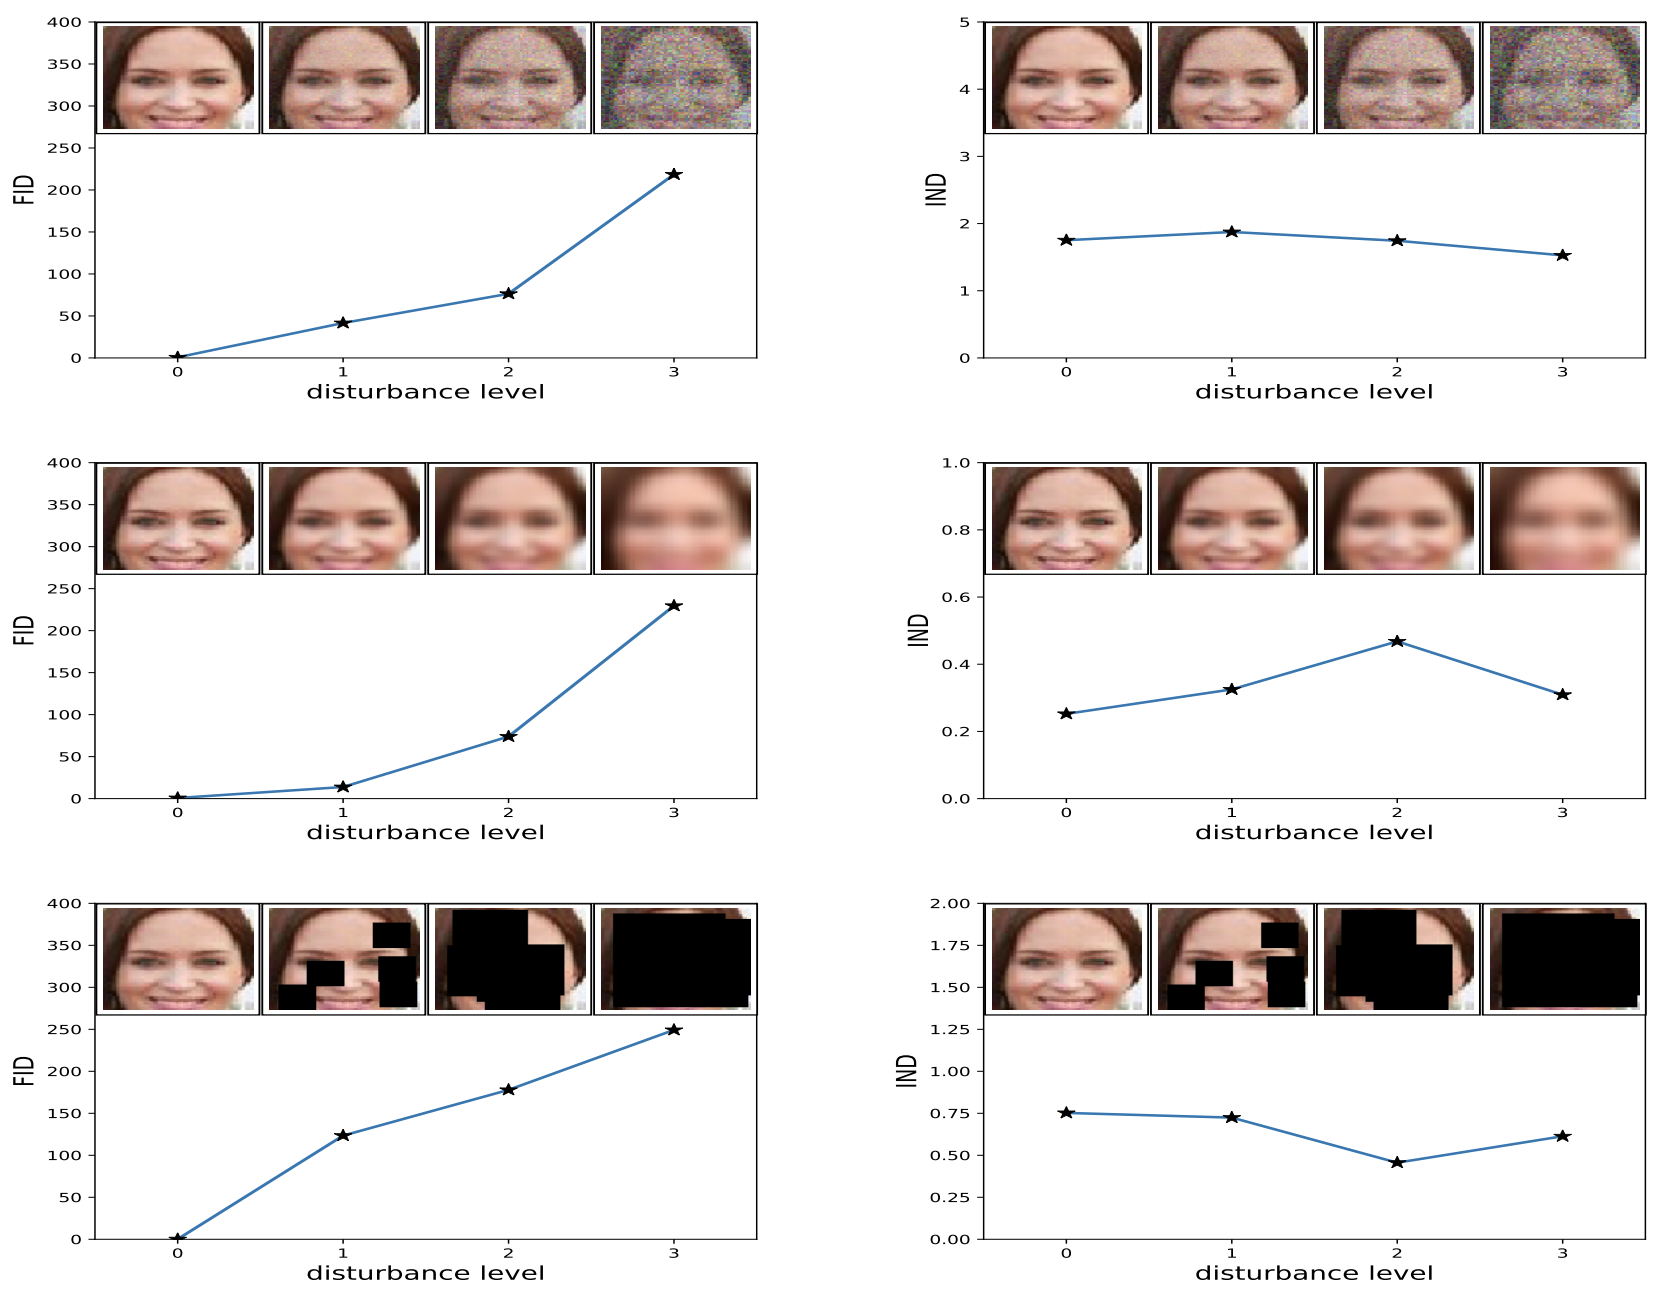
\includegraphics[width=0.9\linewidth]{figs/fid_results}
	\end{figure}
	
	\myfootnotewithlink{https://arxiv.org/abs/1706.08500}{Heusel M. et al. GANs Trained by a Two Time-Scale Update Rule Converge to a Local Nash Equilibrium, 2017}
\end{frame}
%=======
\begin{frame}{Evaluation of likelihood-free models}
	\begin{block}{Frechet Inception Distance}
		\vspace{-0.1cm}
		\[
		D^2 (\pi, p) = \| \mathbf{m}_{\pi} - \mathbf{m}_{p}\|_2^2 + \text{Tr} \left( \bC_{\pi} + \bC_p - 2 \sqrt{\bC_{\pi} \bC_p} \right)
		\]
	\end{block}
	\begin{block}{FID limitations}
		\begin{itemize}
			\item FID depends on the pretrained classification model.
			\item FID needs a large samples  size for evaluation.
			\item Calculation of FID is slow.
			\item FID extimates only two sample moments.
		\end{itemize}
	\end{block}

	\myfootnotewithlink{https://arxiv.org/abs/1706.08500}{Heusel M. et al. GANs Trained by a Two Time-Scale Update Rule Converge to a Local Nash Equilibrium, 2017}
\end{frame}
%=======
\begin{frame}{Summary}
	\begin{itemize}
		\item Wasserstein GAN uses Kantorovich-Rubinstein duality to estimate Wasserstein distance.
		\item Gradient Penalty proposes the regularizer to enforce Lipschitzness.
		\item Spectral normalization is a weight normalization technique to enforce Lipshitzness.
		\item f-divergence family is a unified framework for divergence minimization.
		\item Inception Score and Frechet Inception Distance are the common metrics for GAN evaluation.
	\end{itemize}
\end{frame}
%=======
\begin{frame}{Evolution of GANs}
	\begin{figure}
		\centering
		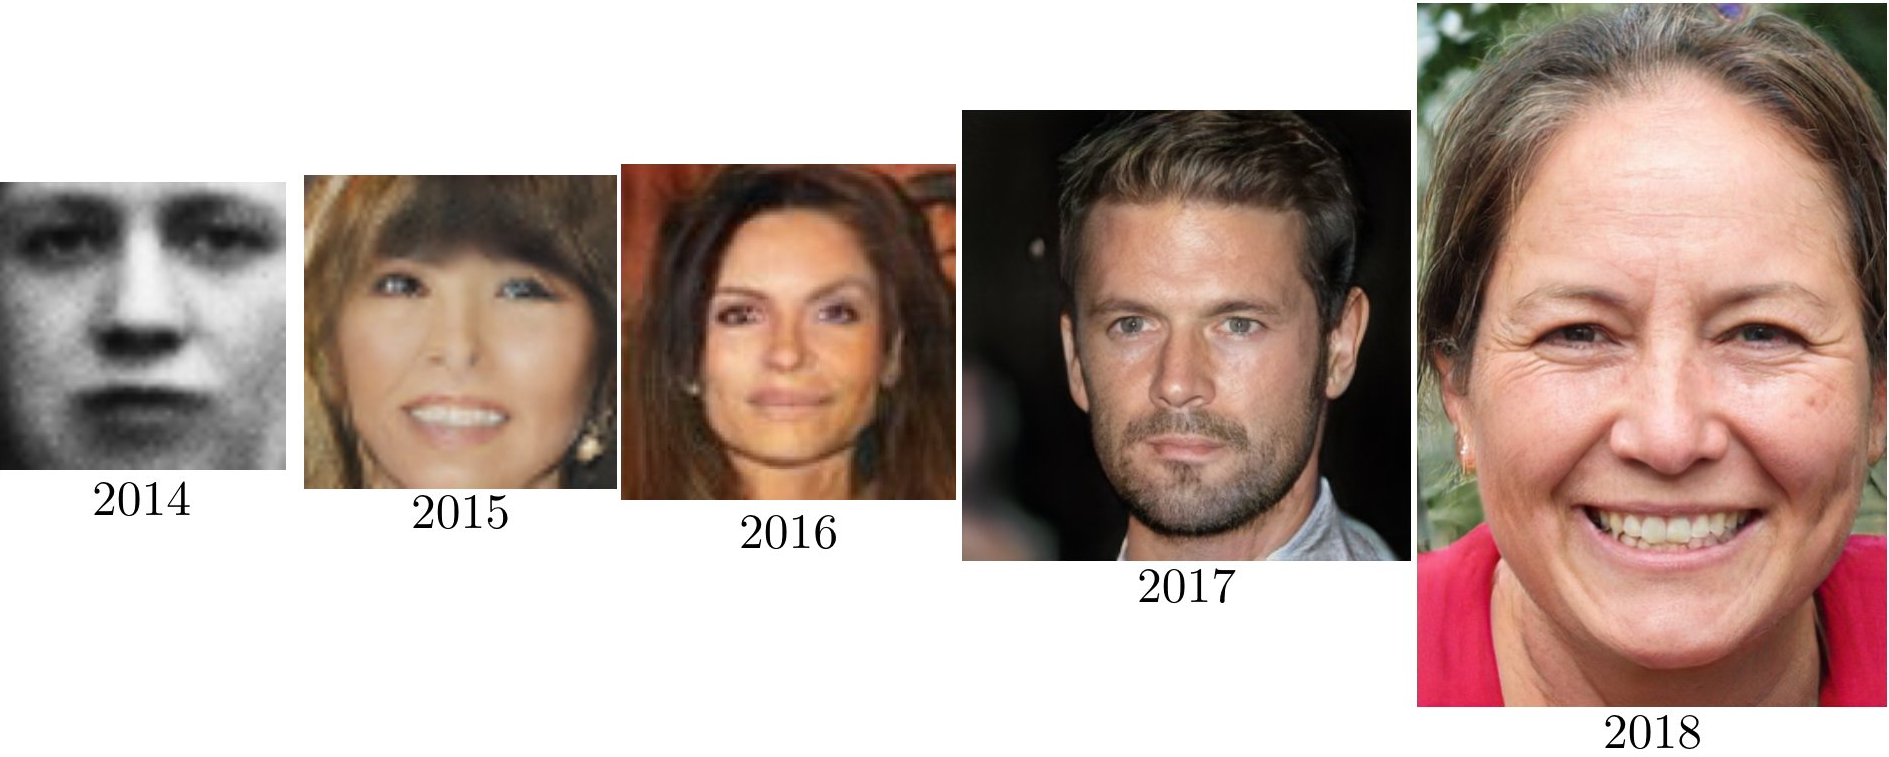
\includegraphics[width=\linewidth]{figs/gan_evolution}
	\end{figure}
	\begin{itemize}
		\item \textbf{Vanilla GAN} \href{https://arxiv.org/abs/1406.2661}{https://arxiv.org/abs/1406.2661}
		\item \textbf{DCGAN} \href{https://arxiv.org/abs/1511.06434}{https://arxiv.org/abs/1511.06434}
		\item \textbf{CoGAN} \href{https://arxiv.org/abs/1606.07536}{https://arxiv.org/abs/1606.07536}
		\item \textbf{ProGAN} \href{https://arxiv.org/abs/1710.10196}{https://arxiv.org/abs/1710.10196} 
		\item \textbf{StyleGAN} \href{https://arxiv.org/abs/1812.04948}{https://arxiv.org/abs/1812.04948}
	\end{itemize}
\end{frame}
%=======
\begin{frame}{Self-Attention GAN}
	\begin{itemize}
		\item Convolutional layers process the information in a local neighborhood.
		\item Using convolutional layers alone is computationally inefficient for modeling long-range dependencies in images.
	\end{itemize}
	\begin{figure}
		\centering
		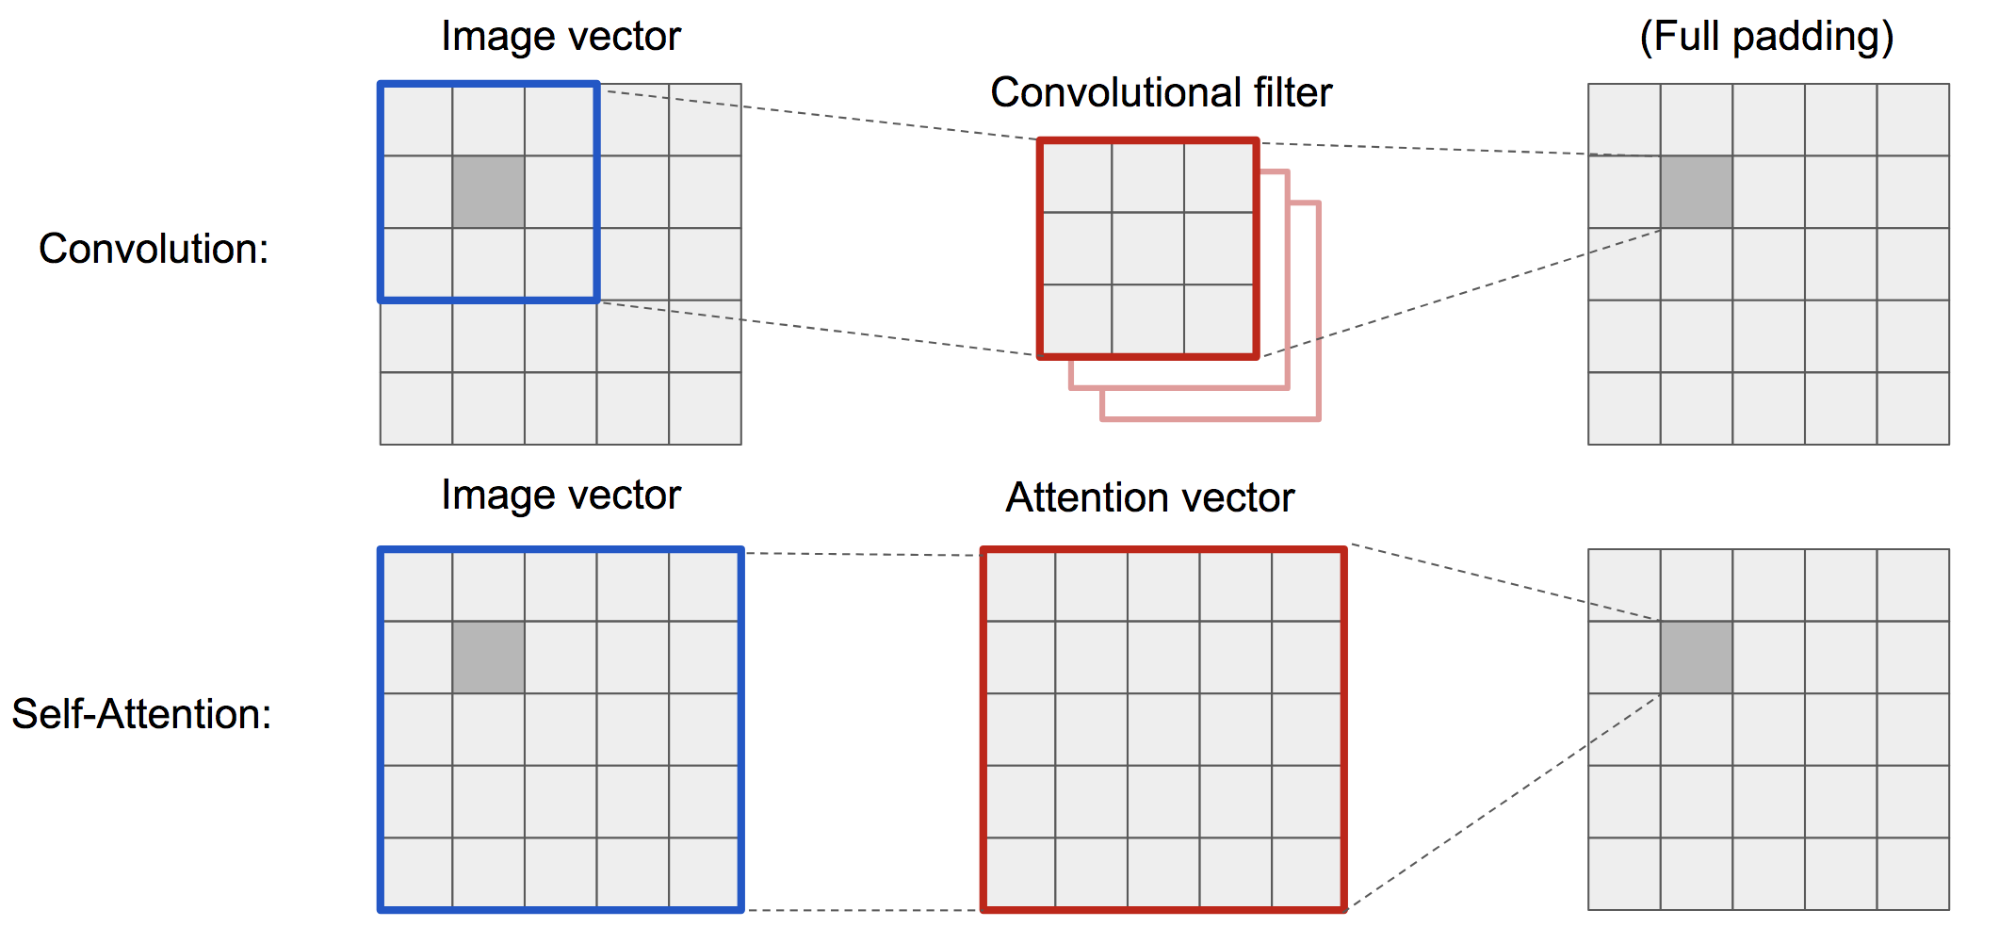
\includegraphics[width=0.9\linewidth]{figs/conv-vs-sa}
	\end{figure}
	\myfootnotewithlink{https://lilianweng.github.io/lil-log/2018/06/24/attention-attention.html}{image credit: https://lilianweng.github.io/lil-log/2018/06/24/attention-attention.html}
\end{frame}
%=======
\begin{frame}{Self-Attention GAN}
	\begin{figure}
		\centering
		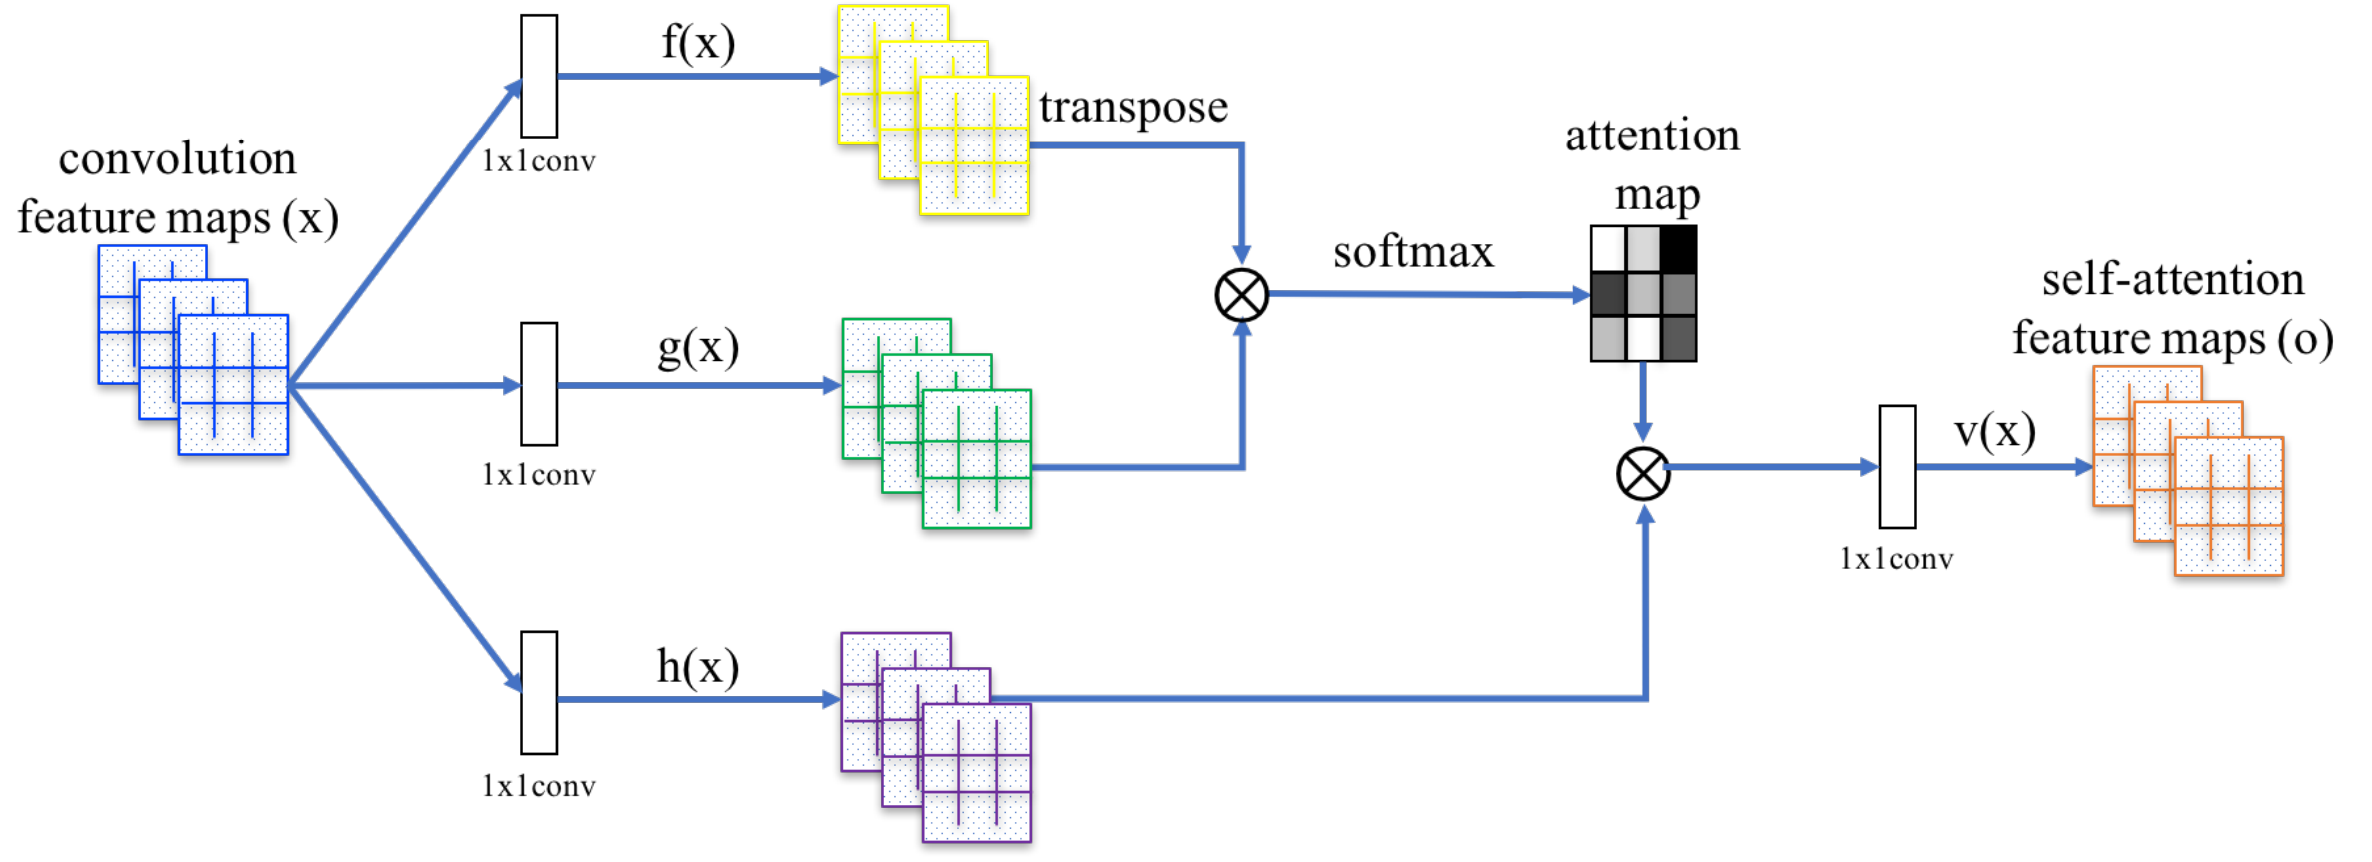
\includegraphics[width=0.9\linewidth]{figs/self-attention}
	\end{figure}
	\vspace{-0.2cm}
	\begin{itemize}
		\item $\bx$ -- feature vector for one feature location.
		\item $N$ -- number of feature locations.
	\end{itemize}
	\vspace{0.5cm}
	\[
		\mathbf{f}(\bx) = \bW_f(\bx), \quad \mathbf{g}(\bx) = \bW_g(\bx), \quad \mathbf{h}(\bx) = \bW_h(\bx), \quad \mathbf{v}(\bx) = \bW_v(\bx)
	\]
	\[
		s_{ij} = \mathbf{f}(\bx_i)^T \mathbf{g}(\bx_j), \quad a_{ij} = \frac{\exp{s_{ij}}}{\sum_{i=1}^N \exp{s_{ij}}}, \quad \textbf{o}_j = \textbf{v}\left( \sum_{i=1}^N a_{ij} \mathbf{h}(\bx_i) \right)
	\]
	\myfootnotewithlink{https://arxiv.org/abs/1805.08318}{Zhang H. et al. Self-Attention Generative Adversarial Networks, 2018}
\end{frame}
%=======
\begin{frame}{Self-Attention GAN}
	\begin{block}{Technical Details}
		\begin{itemize}
			\item Hinge loss for training.
			\item Spectral Normalization in both the generator and the discriminator.
			\item Separate learning rates for the generator and the discriminator.
		\end{itemize}
	\end{block}
	\begin{figure}
		\centering
		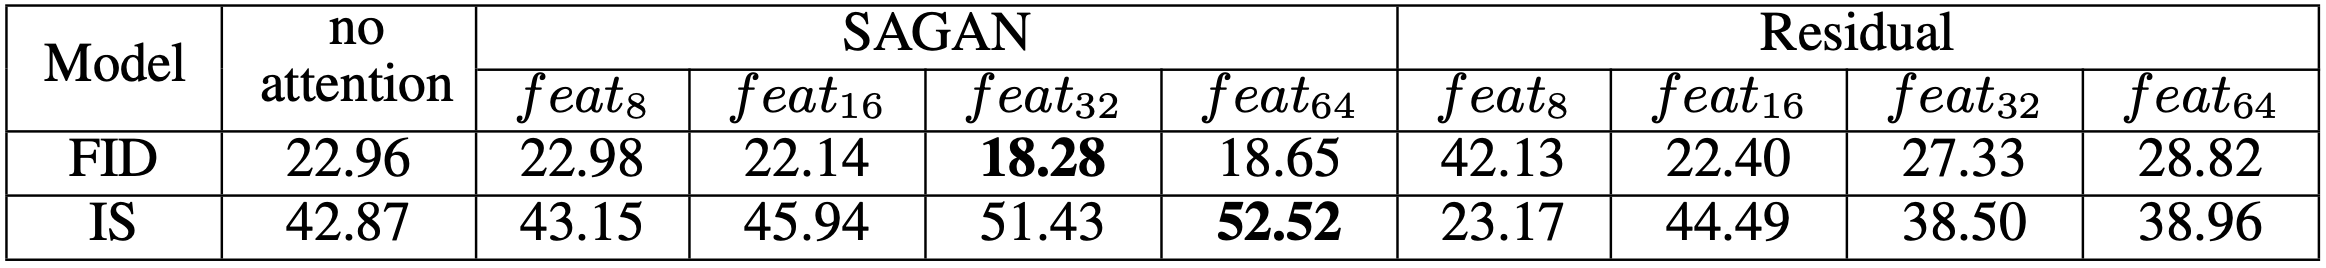
\includegraphics[width=\linewidth]{figs/sa_results1}
	\end{figure}
	\begin{figure}
		\centering
		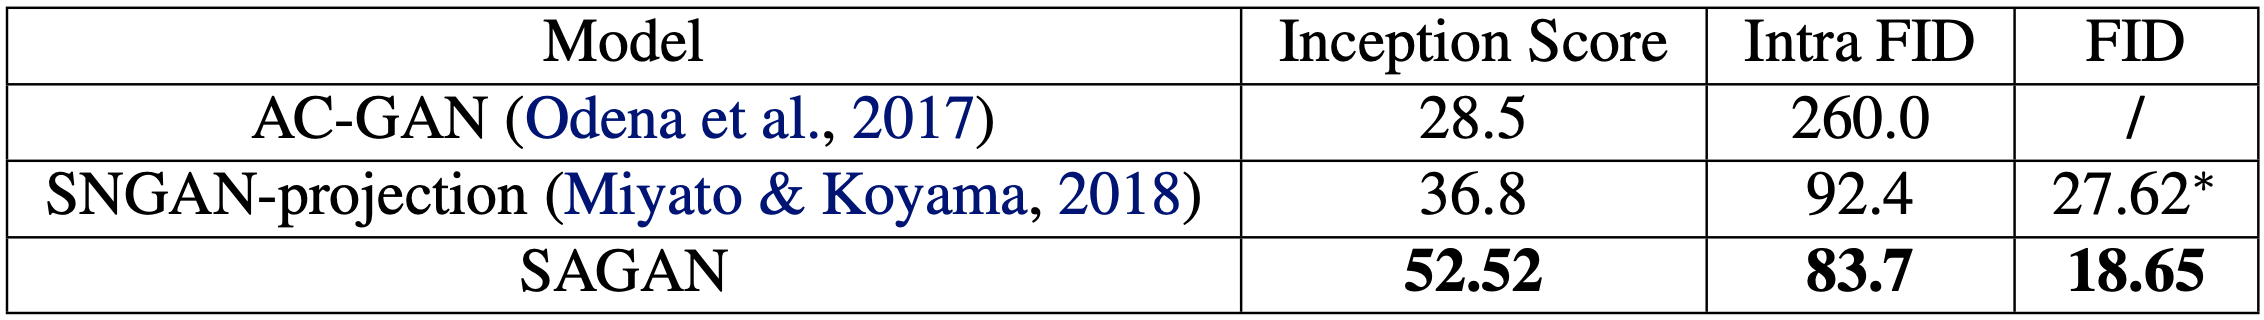
\includegraphics[width=\linewidth]{figs/sa_results2}
	\end{figure}

	\myfootnotewithlink{https://arxiv.org/abs/1805.08318}{Zhang H. et al. Self-Attention Generative Adversarial Networks, 2018}
\end{frame}
%=======
\begin{frame}{Self-Attention GAN}
	\begin{block}{Visualization of attention maps}
		\begin{figure}
			\centering
			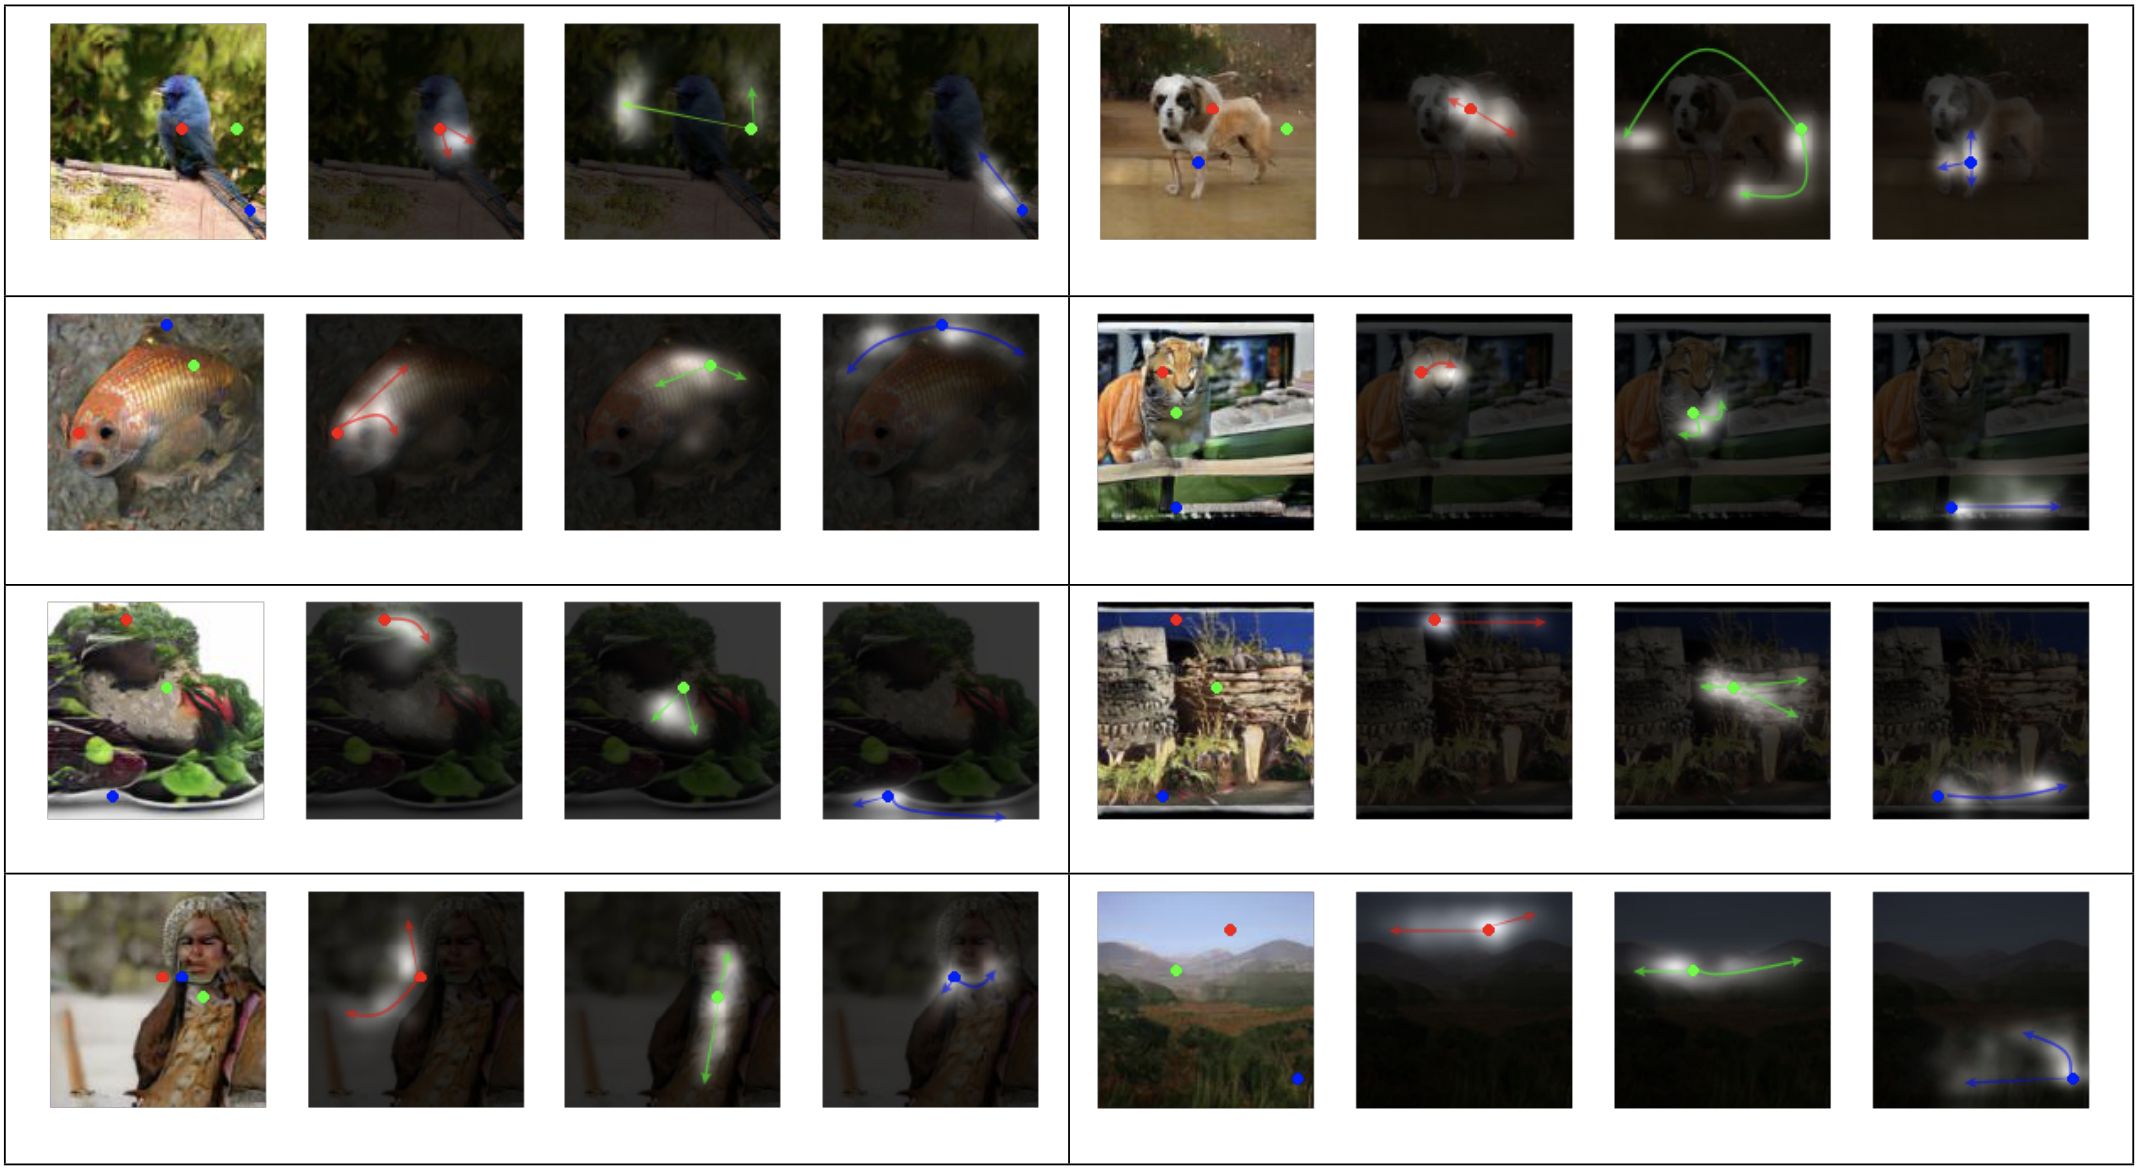
\includegraphics[width=\linewidth]{figs/sa_maps}
		\end{figure}
	\end{block}

	\myfootnotewithlink{https://arxiv.org/abs/1805.08318}{Zhang H. et al. Self-Attention Generative Adversarial Networks, 2018}
\end{frame}
%=======
\begin{frame}{BigGAN}
	\begin{block}{Model description}
		\begin{itemize}
			\item Self-Attention GAN baseline.
			\item Class-conditional generator.
			\item Increasing batch size gives tremendous benefit (allows to cover more modes).
			\item Increasing model size is helpful (wider helps as much as deeper).
			\item Hinge loss for training.
			\item Orthogonal regularization for smoothness the generator output.
			\item Truncation trick for balancing between diversity and fidelity.
		\end{itemize}
	\end{block}
	\vspace{0.5cm}

	\myfootnotewithlink{https://arxiv.org/abs/1809.11096}{Brock A., Donahue J., Simonyan K. Large Scale GAN Training for High Fidelity Natural Image Synthesis, 2018}
\end{frame}
%=======
\begin{frame}{BigGAN}
	\begin{itemize}
		\item \textbf{Orthogonal regularization}
		\[
		\| \bW^T \bW - \bI \|^2 \quad \Rightarrow \| \bW^T \bW - \text{diag}(\bW^T \bW) \|^2
		\]
		\item \textbf{Truncation trick.} Coordinates of samples $\bz \sim \cN(0, \bI)$ which fall outside a predefined range are resampled to fall inside that range.
	\end{itemize}
	\begin{figure}
		\centering
		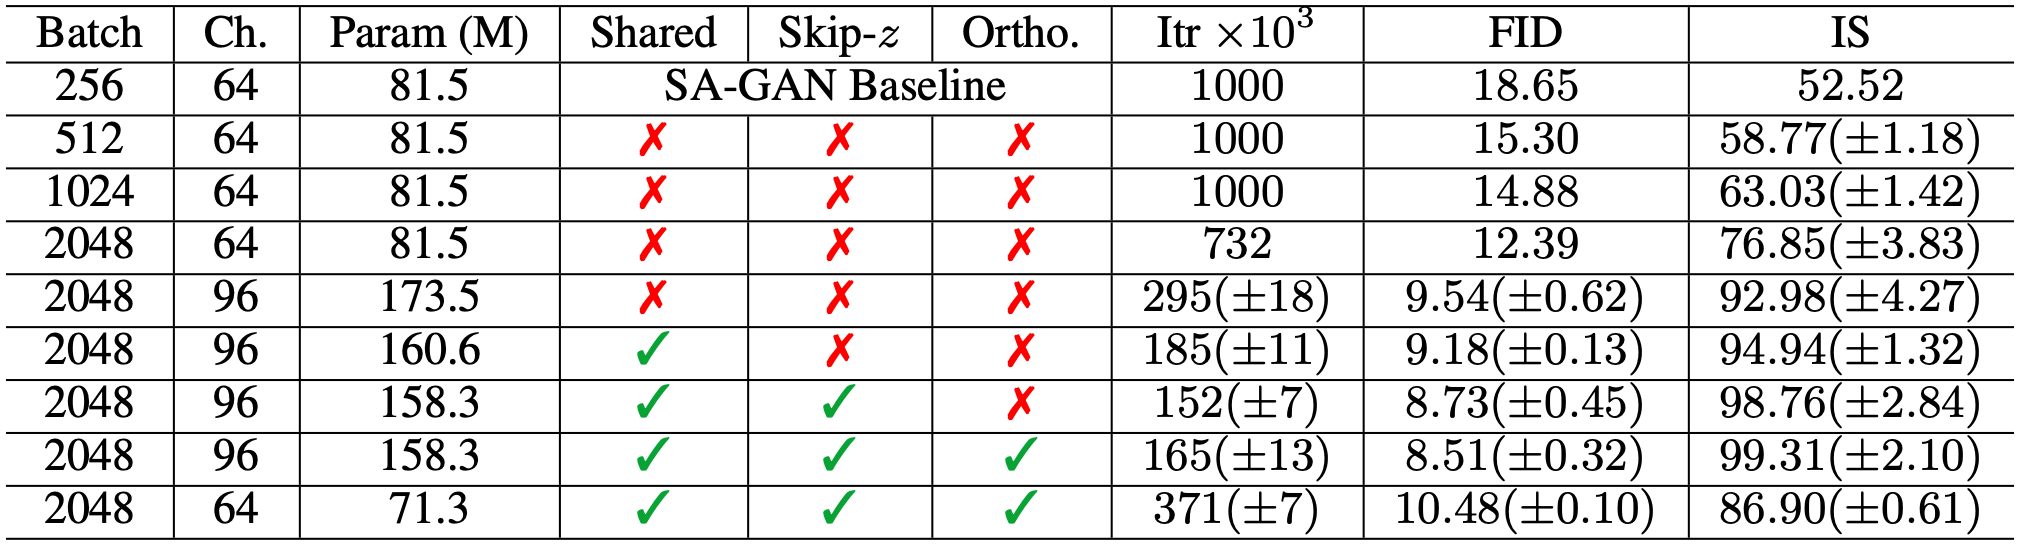
\includegraphics[width=\linewidth]{figs/biggan_results}
	\end{figure}
	
	\myfootnotewithlink{https://arxiv.org/abs/1809.11096}{Brock A., Donahue J., Simonyan K. Large Scale GAN Training for High Fidelity Natural Image Synthesis, 2018}
\end{frame}
%=======
\begin{frame}{BigGAN}
	\begin{block}{Samples (512x512)}
		\begin{figure}
			\centering
			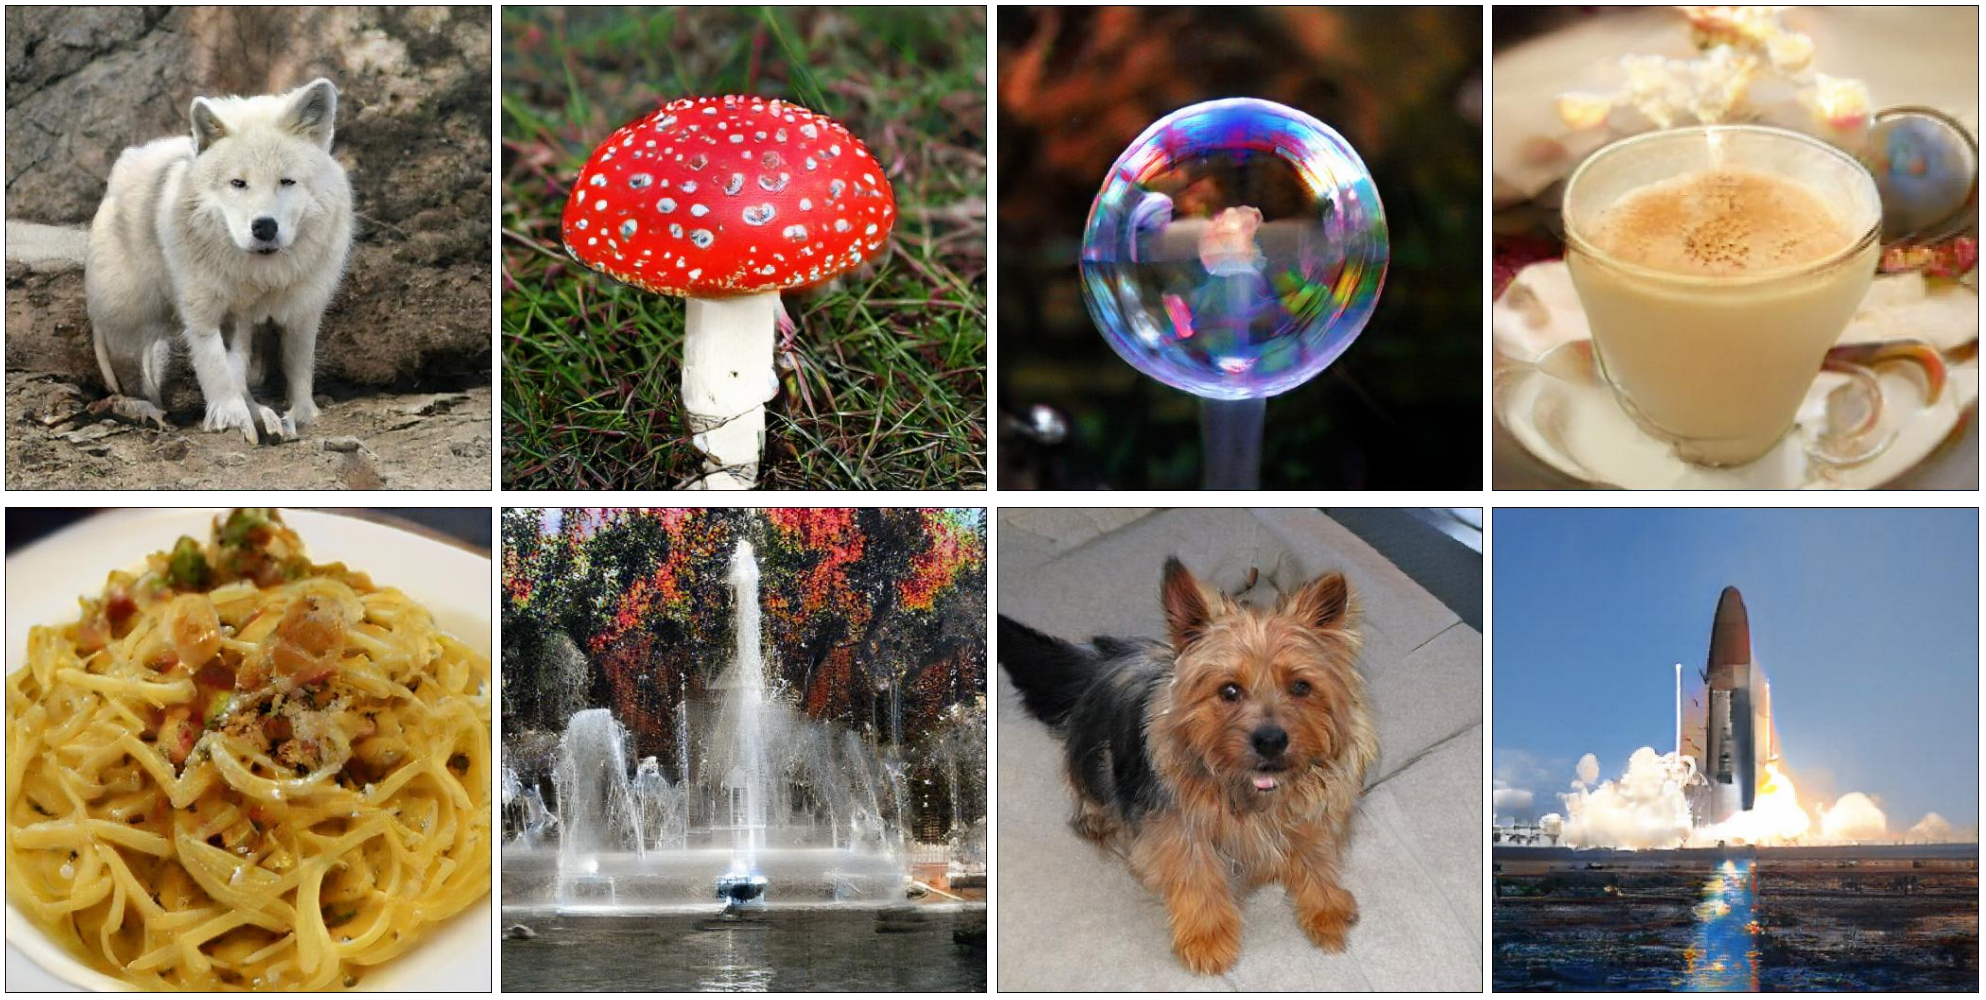
\includegraphics[width=\linewidth]{figs/biggan_samples}
		\end{figure}
	\end{block}
	
	\myfootnotewithlink{https://arxiv.org/abs/1809.11096}{Brock A., Donahue J., Simonyan K. Large Scale GAN Training for High Fidelity Natural Image Synthesis, 2018}
\end{frame}
%=======
\begin{frame}{BigGAN}
	\begin{block}{Interpolations}
		\begin{figure}
			\centering
			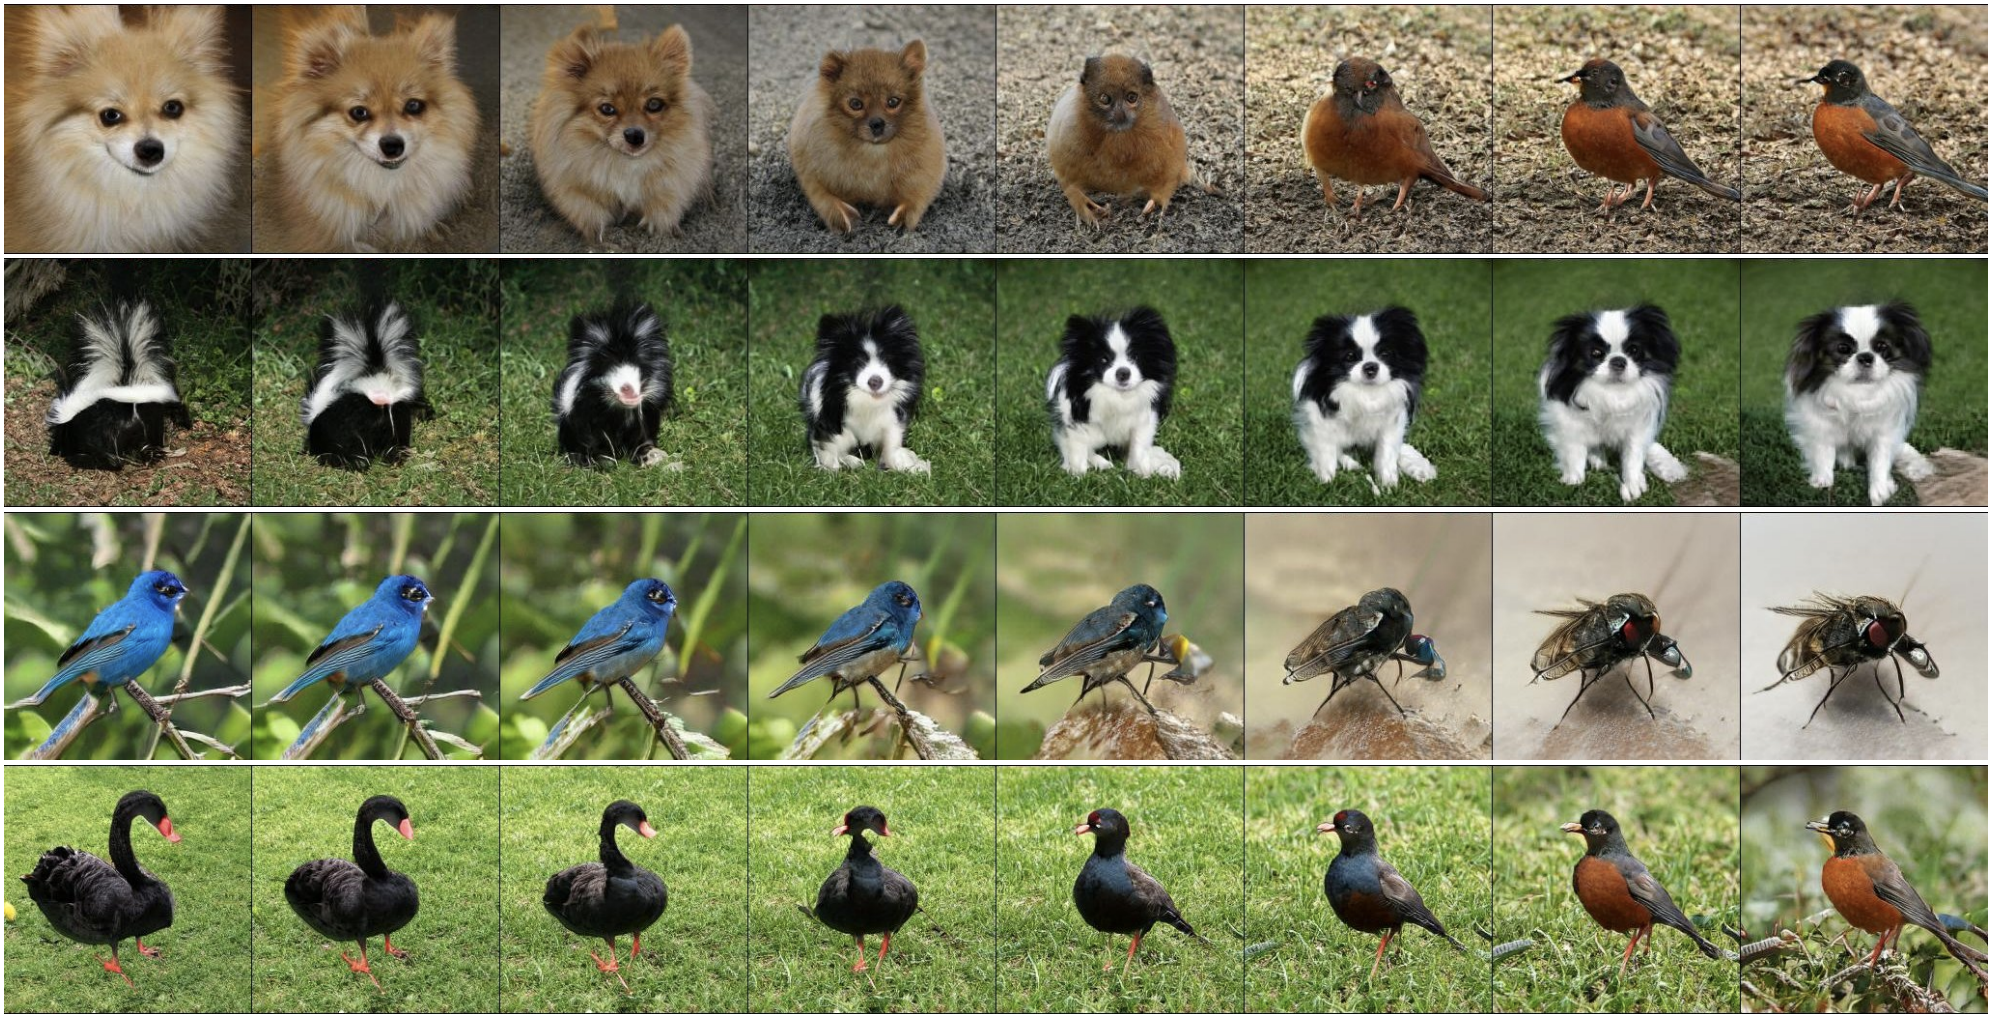
\includegraphics[width=\linewidth]{figs/biggan_interpolations}
		\end{figure}
	\end{block}
	\myfootnotewithlink{https://arxiv.org/abs/1809.11096}{Brock A., Donahue J., Simonyan K. Large Scale GAN Training for High Fidelity Natural Image Synthesis, 2018}
\end{frame}
%=======
\begin{frame}{Progressive Growing GAN}
	\begin{block}{Problems with HR image generation}
		\begin{itemize}
			\item Disjoint manifolds $\Rightarrow$ gradient problem.
			\item Small minibatch $\Rightarrow$ training instability.
		\end{itemize}
	\end{block}
	\begin{block}{Solution}
		Grow both the generator and discriminator progressively, starting from LR images, and add new layers that introduce higher-resolution details as the training progresses. 
		\begin{itemize}
			\item Train GAN which generate 4x4 images (just 2 convolutions for G and D).
			\item Add upsampling layers to G, downsampling layers to D.
			\item Train GAN which generate 8x8 images.
			\item etc.
		\end{itemize}
	\end{block}
	
	\myfootnotewithlink{https://arxiv.org/abs/1710.10196}{Karras T. et al. Progressive Growing of GANs for Improved Quality, Stability, and Variation, 2017}
\end{frame}
\begin{frame}{Progressive Growing GAN}
	\begin{figure}
		\centering
		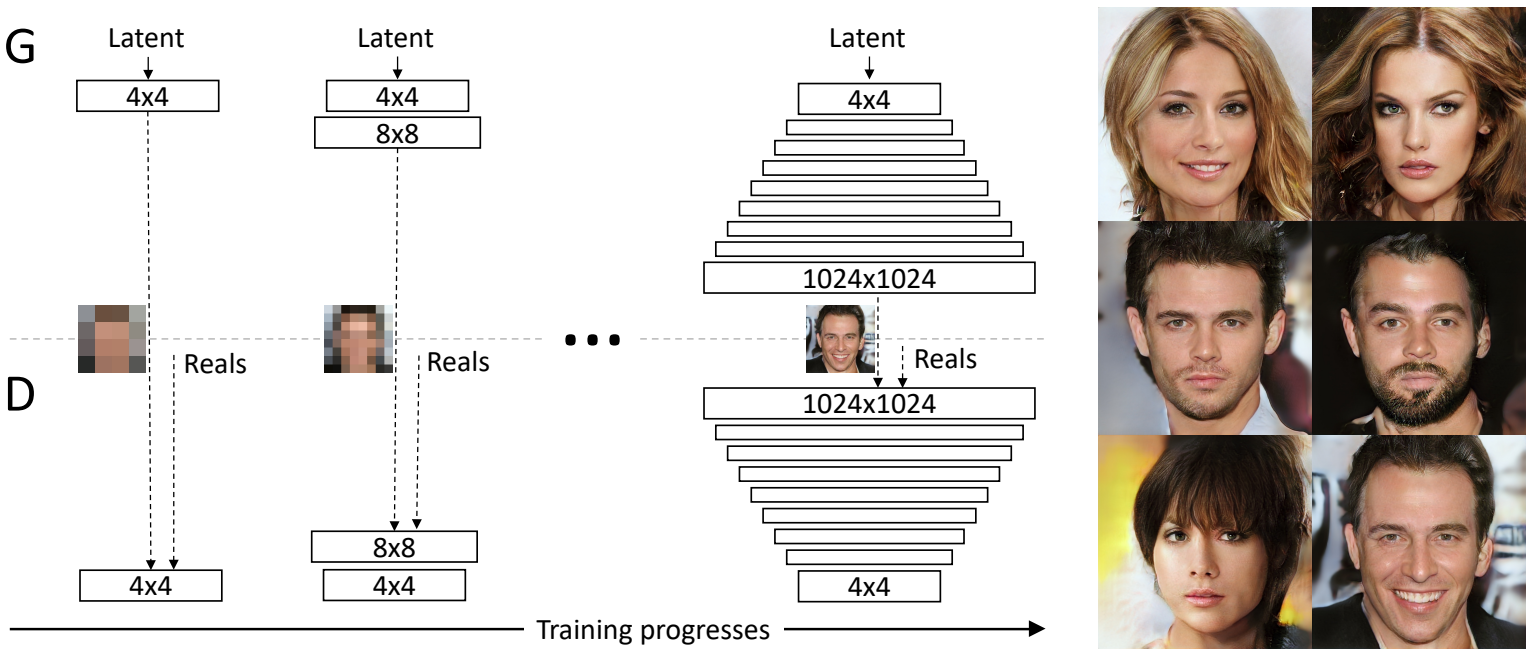
\includegraphics[width=0.8\linewidth]{figs/pggan_arch}
	\end{figure}
	\begin{figure}
		\centering
		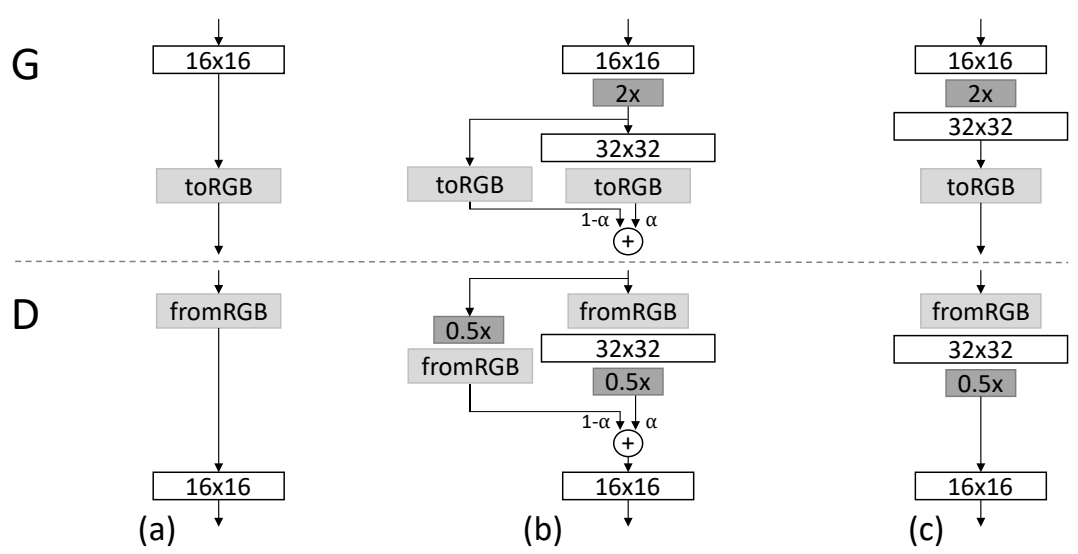
\includegraphics[width=0.6\linewidth]{figs/pggan_fadein}
	\end{figure}

	\myfootnotewithlink{https://arxiv.org/abs/1710.10196}{Karras T. et al. Progressive Growing of GANs for Improved Quality, Stability, and Variation, 2017}
\end{frame}
%=======
\begin{frame}{Progressive Growing GAN}
	\begin{block}{Samples (1024x1024)}
		\begin{figure}
			\centering
			\includegraphics[width=\linewidth]{figs/pggan_samples}
		\end{figure}
	\end{block}

	\myfootnotewithlink{https://arxiv.org/abs/1710.10196}{Karras T. et al. Progressive Growing of GANs for Improved Quality, Stability, and Variation, 2017}
\end{frame}
%=======
\begin{frame}{StyleGAN}
	\begin{itemize}
		\item Generating of HR images is hard.
		\item Progressive growing greatly simplifies the task.
		\item The ability to control specific features of the generated image is very limited.
	\end{itemize}
	\begin{block}{Face image features}
		\begin{itemize}
			\item Coarse (pose, general hair style, face shape). Resolution $4^2 - 8^2$.
			\item Middle (finer facial features, hair style, eyes open/closed). Resolution $16^2 - 32^2$.
			\item Fine (color scheme (eye, hair and skin) and micro features). Resolution $64^2 - 1024^2$.
		\end{itemize}
	\end{block}
	\myfootnotewithlink{https://arxiv.org/abs/1812.04948}{Karras T., Laine S., Aila T. A Style-Based Generator Architecture for Generative Adversarial Networks, 2018}
\end{frame}
%=======
\begin{frame}{StyleGAN}
	\begin{block}{Step 1: Mapping Network}
		\begin{itemize}
			\item Generator input is likely to be \textbf{disentangled}.  Each component of input vector $\bz$ should be responsible for one generative factor.
			\item Mapping network $f: \cZ \rightarrow \cW$ is used to reduce correlations between components of~$\bz$.
		\end{itemize}
		\begin{minipage}[t]{0.6\columnwidth}
			\begin{figure}
				\centering
				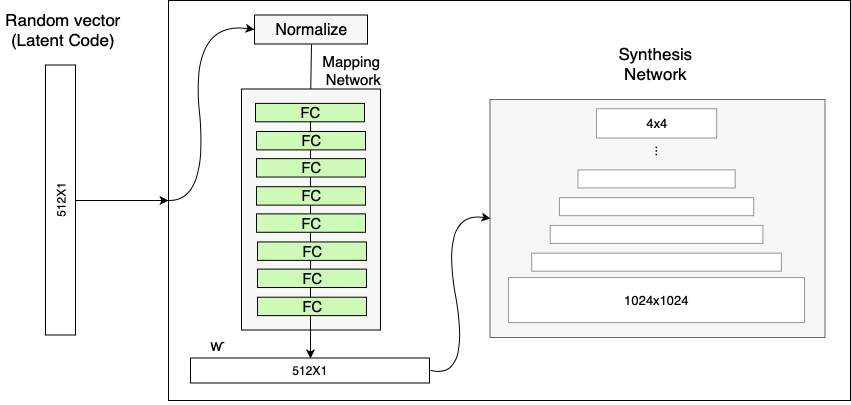
\includegraphics[width=0.98\linewidth]{figs/stylegan_mapping}
			\end{figure}
		\end{minipage}%
		\begin{minipage}[t]{0.38\columnwidth}
			\begin{figure}
				\centering
				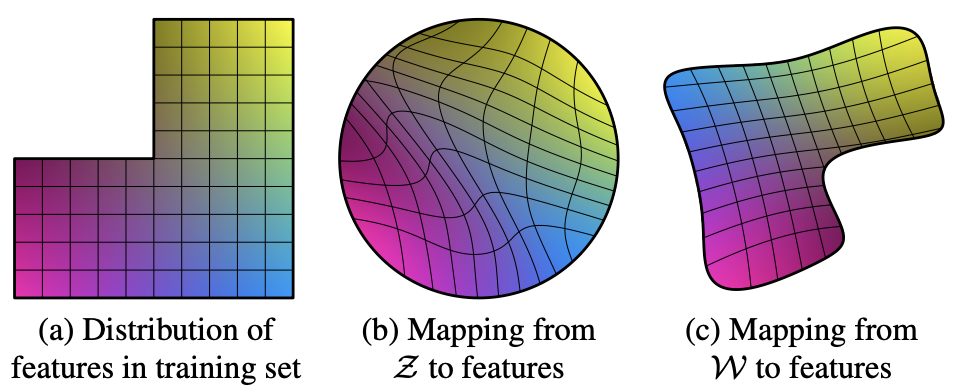
\includegraphics[width=1.0\linewidth]{figs/stylegan_curved}
			\end{figure}
		\end{minipage}
	\vspace{0.3cm}
	\end{block}

	\myfootnotewithlink{https://arxiv.org/abs/1812.04948}{Karras T., Laine S., Aila T. A Style-Based Generator Architecture for Generative Adversarial Networks, 2018}
\end{frame}
%=======
\begin{frame}{StyleGAN}
	\begin{block}{Step 2: Style modulation}
		\begin{itemize}
			\item Adaptive Instance Normalization transfers the $\bw$ vector to the synthesis Network.
			\item The module is added to each resolution to define the visual expression of the features.
		\end{itemize}
		\begin{figure}
			\centering
			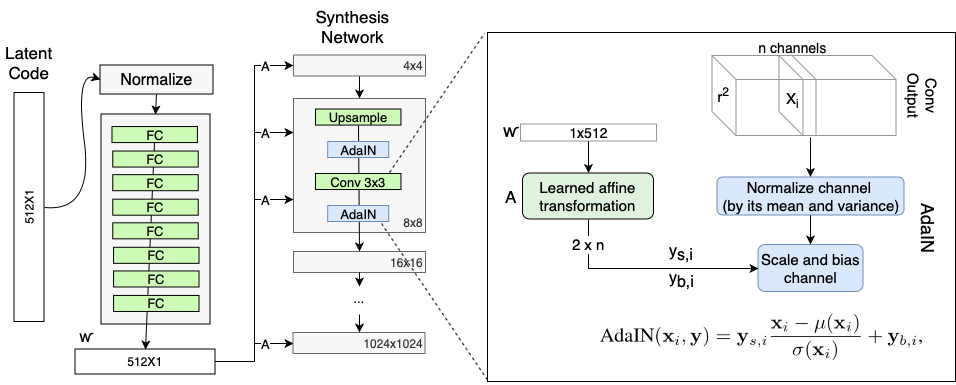
\includegraphics[width=1.0\linewidth]{figs/stylegan_adain}
		\end{figure}
	\end{block}

	\myfootnotewithlink{https://arxiv.org/abs/1812.04948}{Karras T., Laine S., Aila T. A Style-Based Generator Architecture for Generative Adversarial Networks, 2018}
\end{frame}
%=======
\begin{frame}{StyleGAN}
	\begin{block}{Step 3: Remove traditional input}
		Mapping network provides stochasticity to different stages of the synthesis network. Input of the synthesis network is a trainable vector.
		\begin{figure}
			\centering
			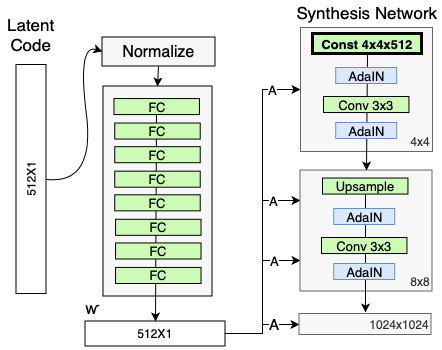
\includegraphics[width=0.55\linewidth]{figs/stylegan_input}
		\end{figure}
	\end{block}

	\myfootnotewithlink{https://arxiv.org/abs/1812.04948}{Karras T., Laine S., Aila T. A Style-Based Generator Architecture for Generative Adversarial Networks, 2018}
\end{frame}
%=======
\begin{frame}{StyleGAN}
	\begin{block}{Step 4: Stochastic variation}
		Inject random noise to add small aspects, such as freckles, exact placement of hairs, wrinkles, features which make the image more realistic and increase the variety of outputs.
		\begin{figure}
			\centering
			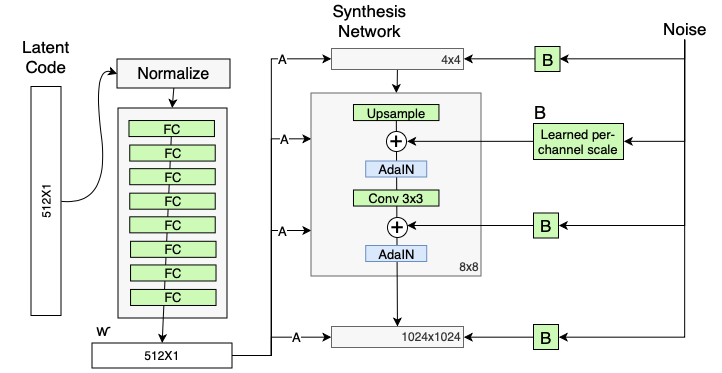
\includegraphics[width=0.9\linewidth]{figs/stylegan_noise}
		\end{figure}
	\end{block}

	\myfootnotewithlink{https://arxiv.org/abs/1812.04948}{Karras T., Laine S., Aila T. A Style-Based Generator Architecture for Generative Adversarial Networks, 2018}
\end{frame}
%=======
\begin{frame}{StyleGAN}
	\begin{block}{Step 4: Style Mixing}
		\vspace{-0.33cm}
		\begin{figure}
			\centering
			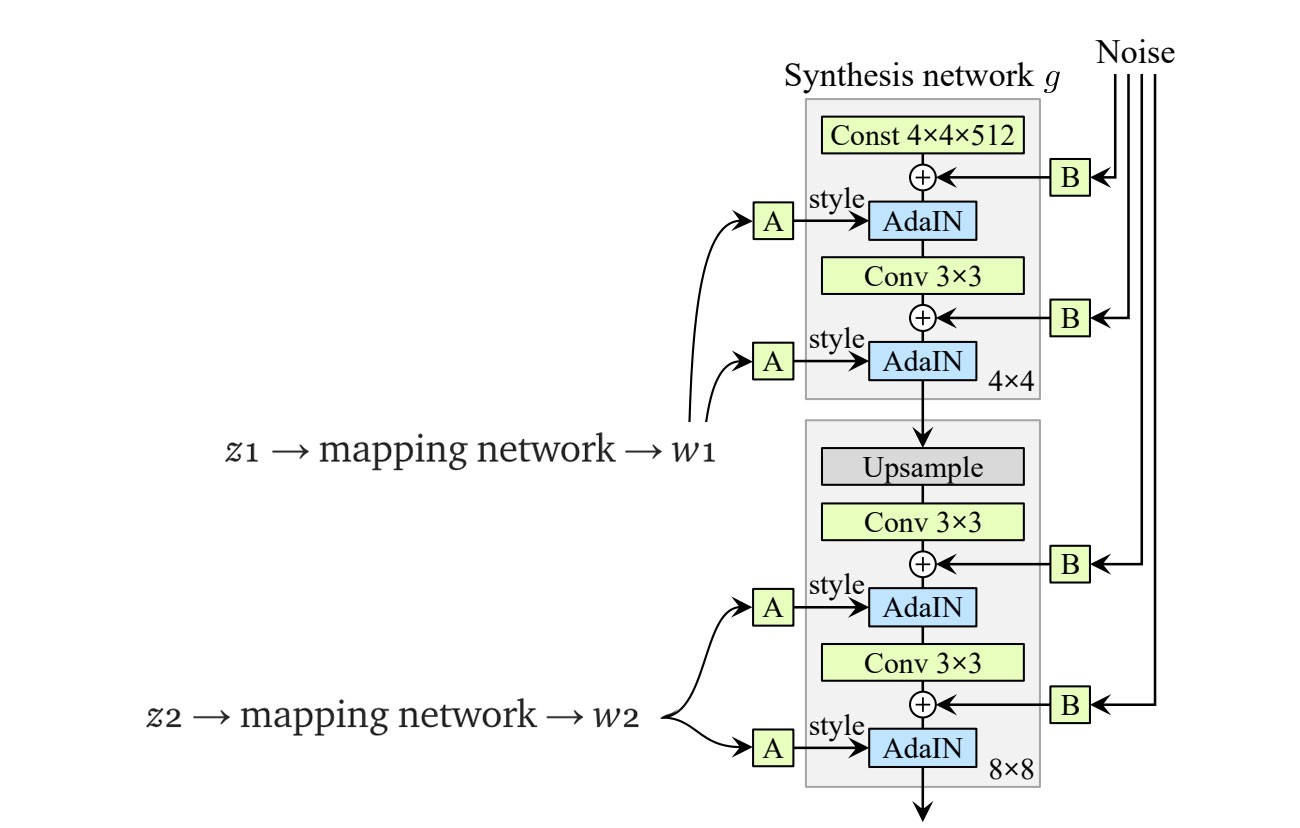
\includegraphics[width=0.8\linewidth]{figs/stylegan_mix_reg}
		\end{figure}
	\begin{itemize}
		\item Makes different levels of synthesis network to be independent.
		\item Allows to couple diffirent styles.
	\end{itemize}
	\end{block}

	\myfootnotewithlink{https://arxiv.org/abs/1812.04948}{Karras T., Laine S., Aila T. A Style-Based Generator Architecture for Generative Adversarial Networks, 2018}
\end{frame}
%=======
\begin{frame}{StyleGAN}
	\begin{figure}
		\centering
		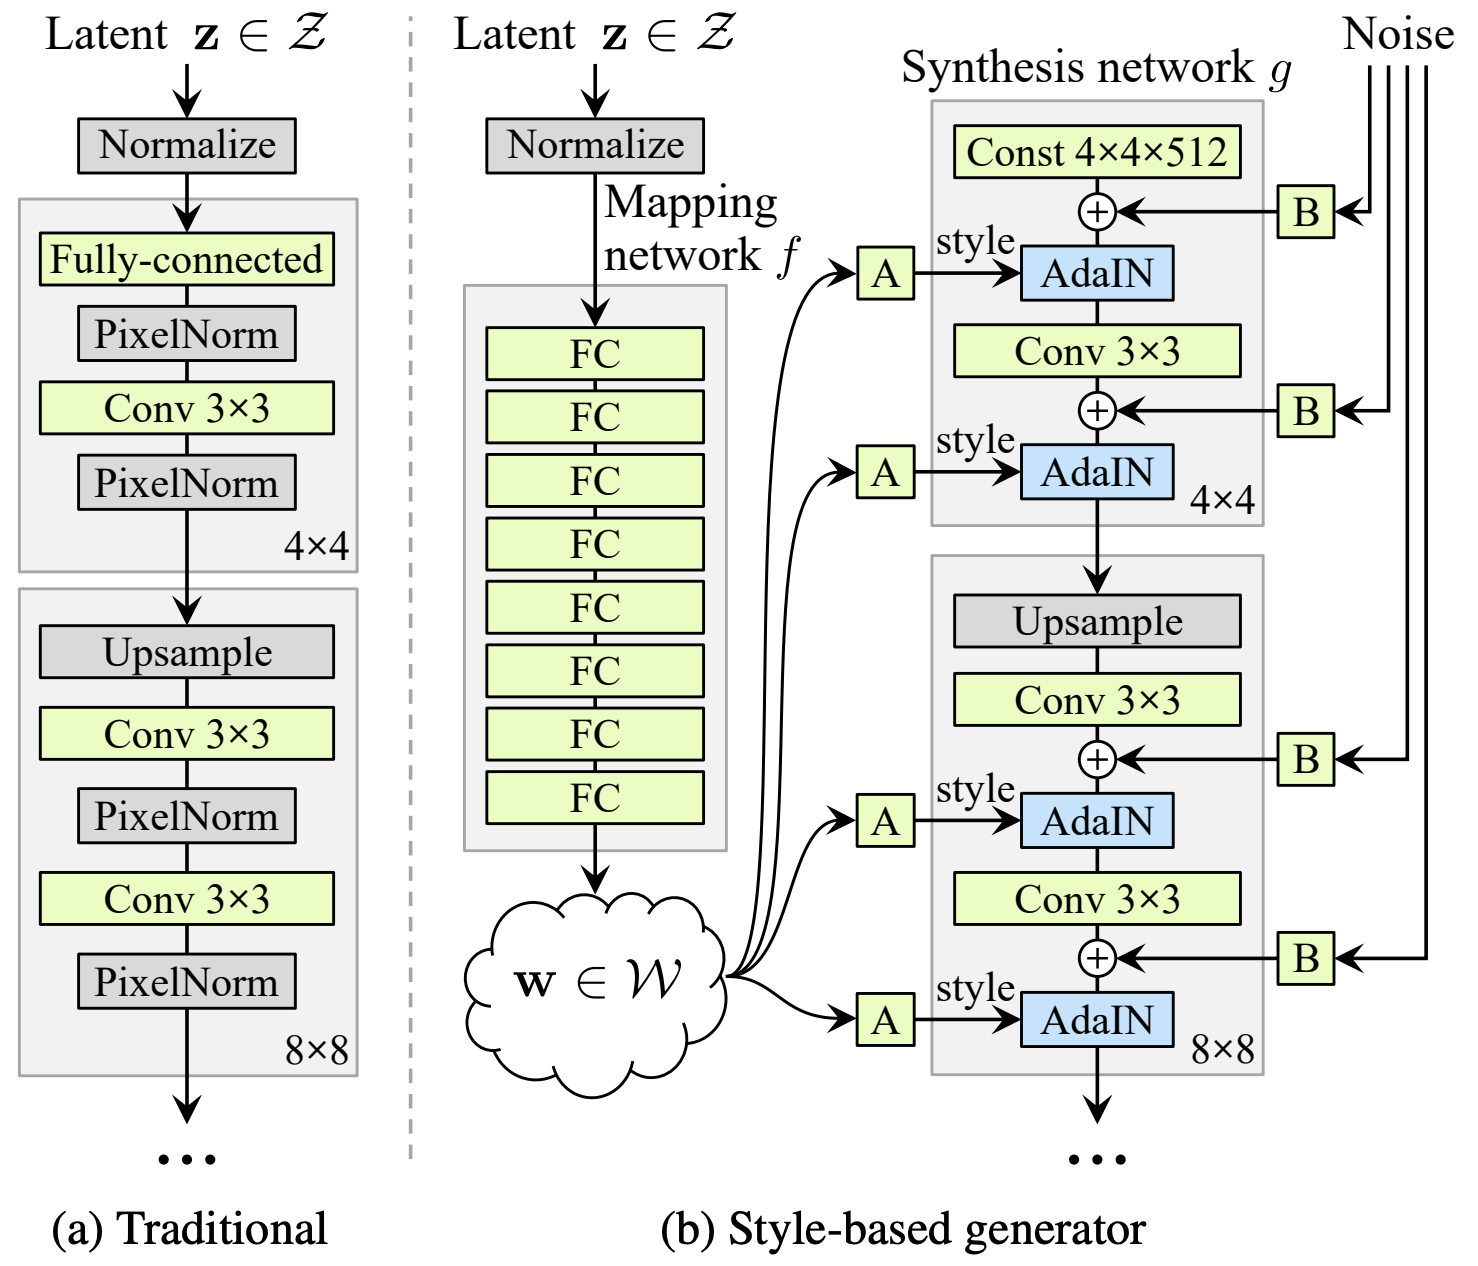
\includegraphics[width=0.8\linewidth]{figs/stylegan_scheme}
	\end{figure}

	\myfootnotewithlink{https://arxiv.org/abs/1812.04948}{Karras T., Laine S., Aila T. A Style-Based Generator Architecture for Generative Adversarial Networks, 2018}
\end{frame}
%=======
\begin{frame}{StyleGAN}
	\begin{block}{Truncation trick}
		\vspace{-0.2cm}
		\[
			\bw' = \hat{\bw} - \psi \cdot (\bw - \hat{\bw}), \quad \hat{\bw} = \bbE_{\bz} p(f(\bz))
		\]
		\vspace{-0.2cm}
		\begin{itemize}
			\item Constant $\psi$ is a tradeoff between diversity and fidelity. 
			\item $\psi=0.7$ is used for most of the results.
			\item Truncation is done only at the low-resolution layers.
		\end{itemize}
		\begin{figure}
			\centering
			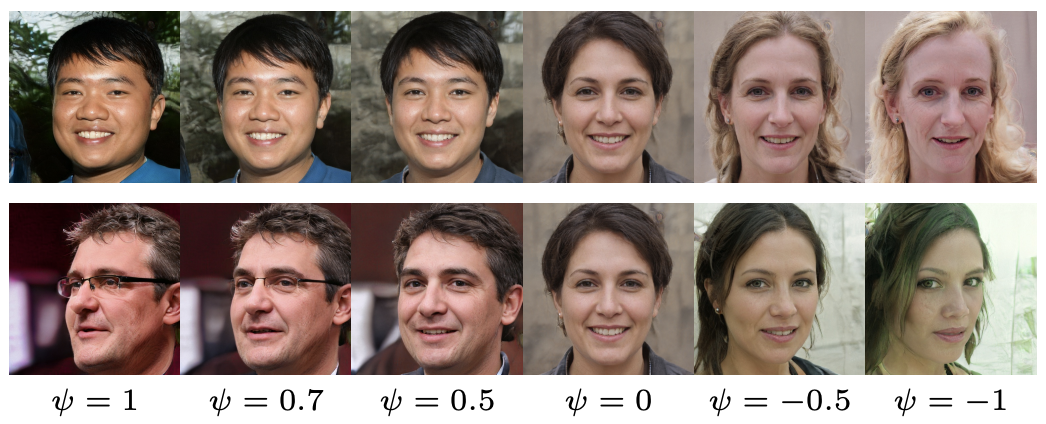
\includegraphics[width=0.8\linewidth]{figs/stylegan_truncation}
		\end{figure}
	\end{block}

	\myfootnotewithlink{https://arxiv.org/abs/1812.04948}{Karras T., Laine S., Aila T. A Style-Based Generator Architecture for Generative Adversarial Networks, 2018}
\end{frame}
%=======
\begin{frame}{StyleGAN}
	\begin{block}{Results}
		\vspace{-0.2cm}
		\begin{figure}
			\centering
			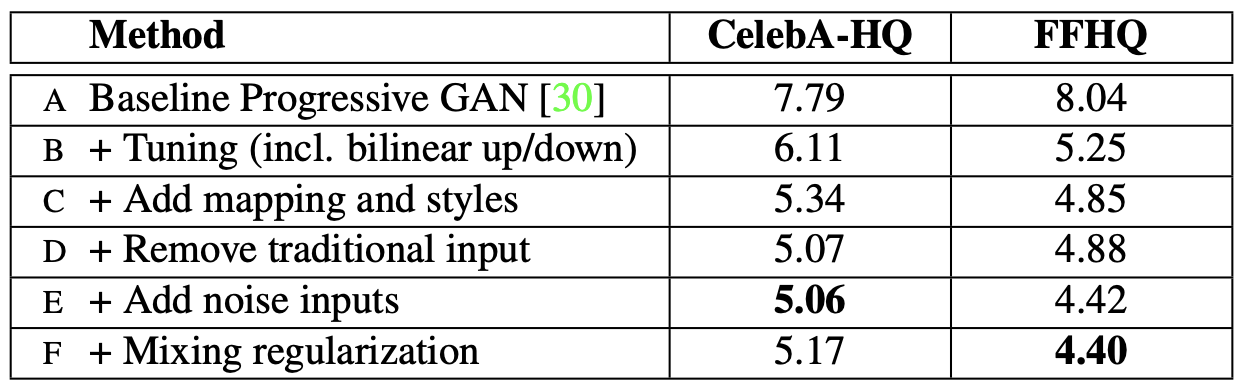
\includegraphics[width=0.6\linewidth]{figs/stylegan_results}
		\end{figure}
	\vspace{-0.3cm}
	\end{block}
	\begin{block}{Samples (1024x1024)}
		\begin{figure}
			\centering
			\includegraphics[width=0.8\linewidth]{figs/stylegan_samples}
		\end{figure}
	\vspace{-0.1cm}
	\end{block}

	\myfootnotewithlink{https://arxiv.org/abs/1812.04948}{Karras T., Laine S., Aila T. A Style-Based Generator Architecture for Generative Adversarial Networks, 2018}
\end{frame}
%=======
\begin{frame}{StyleGAN}
		\begin{figure}
			\centering
			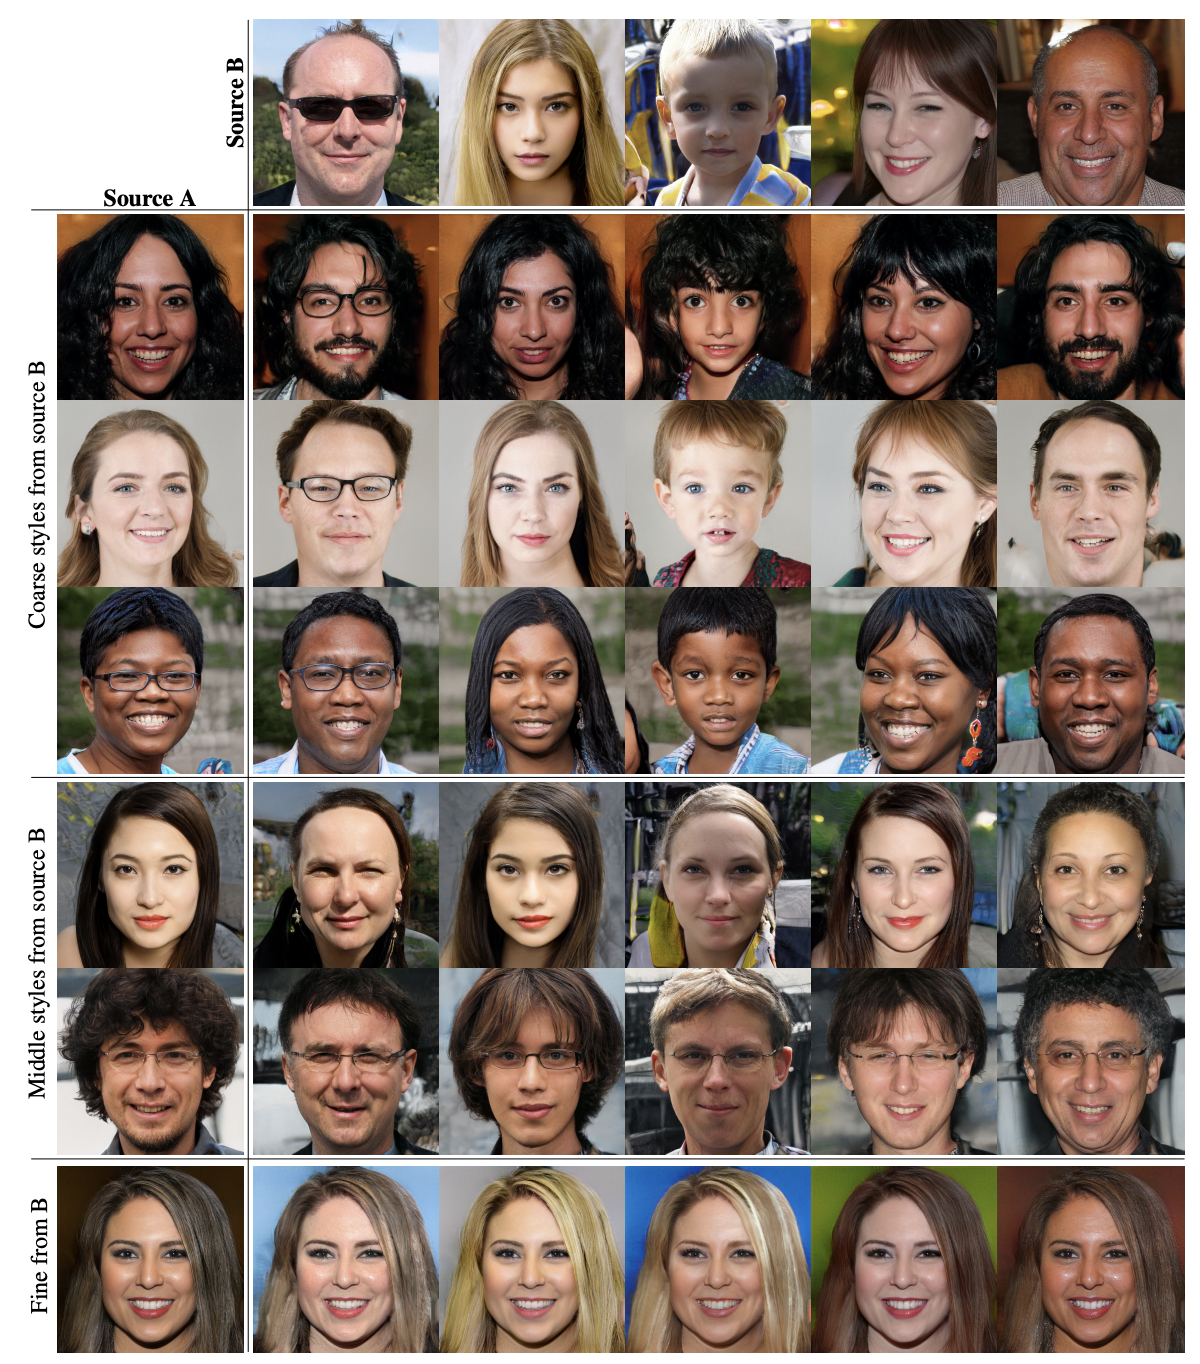
\includegraphics[width=0.6\linewidth]{figs/stylegan_mix}
		\end{figure}

	\myfootnotewithlink{https://arxiv.org/abs/1812.04948}{Karras T., Laine S., Aila T. A Style-Based Generator Architecture for Generative Adversarial Networks, 2018}
\end{frame}
%=======
\begin{frame}{Summary}
\end{frame}
%=======
\end{document} 